\documentclass[10pt,a4paper]{article}
\usepackage{amsmath} % Advanced math typesetting
\usepackage{polski}
\usepackage[utf8]{inputenc} % Unicode support (Umlauts etc.)
\usepackage{graphicx} % Add pictures to your document
\usepackage{listings} % Source code formatting and highlighting
\usepackage{amsfonts}
\usepackage{amssymb}
\usepackage{indentfirst}
\usepackage{graphicx}
\usepackage{url}
\usepackage[polish]{babel} %język polski
%%% fix for \lll - żeby działało amssymb
\let\babellll\lll
\let\lll\relax
\usepackage[T1]{fontenc} %europejski układ fontów
\usepackage{lmodern} %razem z T1 żeby ładnie wyglądały czcionki
\usepackage{wrapfig} %opływanie tekstem grafiki
\usepackage{placeins} %żeby działało \FloatBarrier
\usepackage{color}  %żeby działały kolory :)
\usepackage[usenames,dvipsnames]{xcolor}
\usepackage{enumerate}
\usepackage{geometry}
\usepackage{pdflscape}

\title{
	
\includegraphics[width=6cm]{logoAGH}\\
	\bigskip {Detekcja zespołów QRS} \bigskip	
}
\author{
Monika Daniec,\\
Arkadiusz Jabłoński,\\
Karolina Jedlińska,\\
Anna Kica,\\
Kinga Kraj,\\
Aleksandra Kunowska,\\
Paulina Podłęcka,\\
Aleksandra Sołtysik,\\
Przemysław Węgrzynowicz,\\
Agnieszka Żądło
}
\date{\bigskip \bigskip Kraków, 2017r.}

\begin{document}
\maketitle
\newpage
\tableofcontents

\newpage
\section{Wstęp}

Serce ma za zadanie tłoczenie krwi z naczyń żylnych, w których panuje niskie ciśnienie, do naczyń tętniczych, wskutek czego w tych ostatnich wzrasta ciśnienie. W tym celu konieczne są stałe, rytmiczne skurcze serca, wywoływane zjawiskami elektrycznymi, które można badać przy pomocy elektrokardiografu. Zapis czynności bioelektrycznej serca nazywany jest elektrokardiogramem. \cite{Hoser} Przykładowy zapis takiego sygnału zaprezentowano na Rys.\ref{QRS}.

\medskip
\begin{figure}[h]
\centering
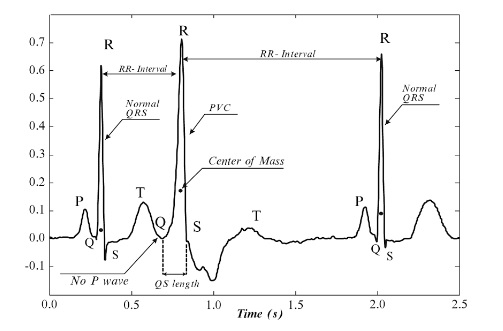
\includegraphics[width=\textwidth]{QRS}
\caption{Przykładowy zapis sygnału EKG wraz z oznaczonymi załamkami. \cite{obrazek} }
\label{QRS}
\end{figure} 
\medskip

Do charakterystycznych cech sygnału EKG należą: załamek P, zespół załamków QRS oraz załamek T. Załamek P odpowiada za elektryczną akcję przedsionków, zespół QRS - skurcz komór, natomiast załamek T reprezentuje proces repolaryzacji.\cite{EKG dla praktyka}

Detekcja oraz określenie granic załamków jest istotnym elementem analizy cyfrowych elektrokardiogramów. Na podstawie wyznaczonych miejsc występowania odpowiednich załamków istnieje możliwość klasyfikacji zespołów czy diagnostyki odcinków ST i QT oraz załamka P. \cite{lab}

Algorytmy odpowiadające za detekcję zespołów QRS są nadal rozwijane i udoskonalane. W niniejszym przedstawiono wybrane rozwiązania.

\newpage
\begin{thebibliography}{9}
\bibitem{Hoser} P. Hoser: \emph{Fizjologia organizmów z elementami anatomii człowieka}, Warszawa, WSiP, 1996, s. 195-197.
\bibitem{obrazek} A. Gacek, W. Pedrycz, \emph{ECG Signal Processing Classification and Interpretation : A Comprehensive Framework of Computational Intelligence} [w:] \url{https://books.google.pl/books?id=lPTiGqPKY94C&pg=PA108&redir_esc=y#v=onepa
ge&q&f=false} s.1018 (dostęp 21.12.2016r.).
\bibitem{EKG dla praktyka} P. Augustyniak, \emph{Elektrokardiografia dla informatyka - praktyka}, Kraków, Wydawnictwo Studenckiego Towarzystwo Naukowego, 2011, s.144-146.
\bibitem{lab} T. Pięciak, [w:] \url{http://home.agh.edu.pl/~pieciak/SygnalyBiomedyczne/laboratorium_ekg.pdf} (dostęp: 21.12.2016r.).

\end{thebibliography}
\newpage
\section{Difference Operation Method}
\subsection{Cel projektu}

Celem projektu była implementacja algorytmu detekcji załamków QRS w sygnale EKG za pomocą algorytmu Difference Operation Method (DOM). 

\subsection{Opis algorytmu}\cite{domB1}

Algorytm DOM składa się z dwóch etapów: przetwarzania sygnału oraz detekcji fal. Przetwarzanie sygnału ma na celu wzmocnienie zespołów QRS w sygnale i osłabienie pozostałych jego części. Natomiast detekcja fal polega na wyszukaniu i zapisie miejsc występowania zespołów QRS w zarejestrowanym sygnale.

Pierwszym krokiem przetwarzania jest filtracja sygnału EKG, na którą składają się 4 etapy:

\begin{itemize}
	\item Filtracja filtrem pasmowo – zaporowym o częstotliwości odcięcia: 60 Hz. Operacja ta ma na celu zredukowanie zakłóceń pochodzących z sieci zasilającej
	\item Filtracja filtrem górnoprzepustowym o częstotliwości odcięcia: 0.5 Hz. Ma to na celu usunięcie pływającej linii izoelektrycznej
	\item Filtracja filtrem morfologicznym – operacja otwarcia oraz zamknięcia przy użyciu elementu strukturalnego (sygnału prostokątnego o zadanej długości) 
	\item Filtracja filtrem adaptacyjnym w celu usunięcia zakłóceń spowodowanych przemieszczeniem elektrod podczas badania
\end{itemize}

Następnie otrzymywany jest sygnał różnicowy , zgodnie z równaniem ~\ref{eq:domE1}:

\begin{equation} \label{eq:domE1}
	x_d(n)=x_d(n)-x_d(n-1)
\end{equation}

Gdzie:

\begin{itemize}
	\item $x(n)$ – sygnał wejściowy w czasie n
	\item $x_d(n)$ – wyjściowy sygnał różnicowy w czasie n
\end{itemize}

Sygnał oryginalny oraz po operacji różnicowania znajdują się odpowiednio na rysunkach ~\ref{fig:dom1} i ~\ref{fig:dom2}.

\begin{figure}
  	\centering
    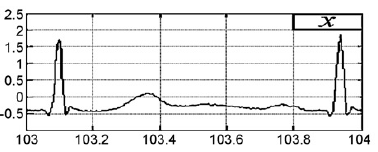
\includegraphics{dom1}
    \caption{Oryginalny sygnał EKG}
  	\label{fig:dom1}
\end{figure}

\begin{figure}
  	\centering
    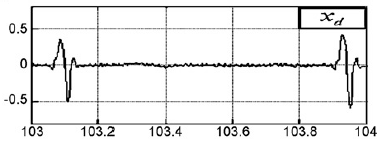
\includegraphics{dom2}
    \caption{Sygnał EKG po operacji różnicowania}
  	\label{fig:dom2}
\end{figure}

Następnym etapem jest filtracja filtrem dolnoprzepustowym o częstotliwości odcięcia 100 Hz, aby usunąć fale o niskiej amplitudzie i wysokiej częstotliwości obecne w sygnale różnicowym. Wynikowy sygnał jest oznaczany jako $x_df$. Sygnał po filtracji jest widoczny na rysunku ~\ref{fig:dom3}.

\begin{figure}
  	\centering
    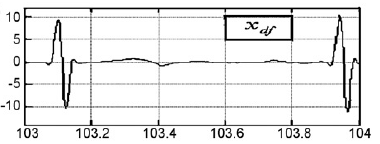
\includegraphics{dom3}
    \caption{Sygnał EKG po operacji filtracji dolnoprzepustowej}
  	\label{fig:dom3}
\end{figure}

Dalszym krokiem jest progowanie sygnału, zgodnie z formułą ~\ref{eq:domE2}:

\begin{equation} \label{eq:domE2}
	\hat{x}_{df} = \left\{ \begin{array}{ll}
	0 & \textrm{dla $0<x_{df}<T_1 \quad lub \quad T_2<x_{df}<0$}\\
	x_{df} & \textrm{dla $x_{df}\geq T_1 \quad lub \quad x_{df} \leq T_2$}
	\end{array} \right.
\end{equation}

Gdzie:

\begin{itemize}
	\item $T_1$ = $2*MV_P$ ($MV_P$ – średnia wartość dodatnich amplitud w całym sygnale)
	\item $T_2$ = $2*MV_N$ ($MV_N$ – średnia wartość ujemnych amplitud w całym sygnale)
\end{itemize}

Sygnał EKG po operacji progowania znajduje się na rysunku ~\ref{fig:dom4}. Kolejno wykonano schemat powyższych czynności w języku UML (rysunek ~\ref{fig:dom5}). Po otrzymaniu sygnału $\hat{x}_{df}$, dokonywana jest detekcja zespołów QRS w następujących etapach: 

\begin{figure}
  	\centering
    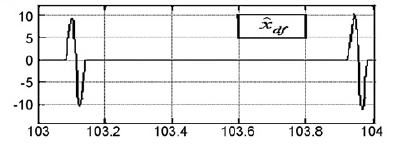
\includegraphics{dom4}
    \caption{Sygnał po operacji progowania.}
  	\label{fig:dom4}
\end{figure}

\begin{figure}
  	\centering
    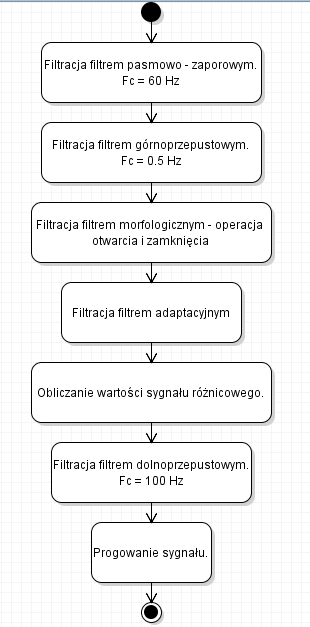
\includegraphics{dom5}
    \caption{Schemat przetwarzania sygnału.}
 	 \label{fig:dom5}
\end{figure}
	
\begin{itemize}
	\item 	Sygnał jest dzielony na dwa sygnały: dodatni $\hat{x}_{df}^+$ oraz ujemny $\hat{x}_{df}^-$
	\item Sygnały dodatni i ujemny są dzielone na interwały o długości 50 próbek (dla częstotliwości próbkowania 360 Hz). W związku z tym czas trwania pojedynczego interwału wynosi 0.14s. Wybierane i zapisywane są te interwały, w których znajduje się przynajmniej jedna niezerowa wartość. Pozostałe interwały są ignorowane.
	\item Na podstawie odległości między dwoma kolejnymi interwałami zawierającymi wartości niezerowe, następuje przyporządkowanie ekstremów do jednej z dwóch grup:

	\begin{itemize}
		
	\item Jeżeli odległość jest mniejsza lub równa długości interwału (0.14s), to spośród dwóch wartości wybierana jest większa z nich. Przykładowo na rysunku ~\ref{fig:dom6}, punkty A i B są maksimami w interwałach odpowiednio  i-1 oraz i. Wybrany zostaje punkt B, ze względu na jego większą wartość
	\item Jeżeli odległość jest większa od długości interwału, to obie wartości są wybierane. Przykładowo na rysunku ~\ref{fig:dom6}, punkty B i C są maksimami interwałów odpowiednio i oraz j. Odległość między punktami B i C jest większa od długości interwału, a zatem oba punkty zostają wybrane do dalszej analizy
		
	\end{itemize}
	\item Na podstawie odległości między ekstremami sygnałów dodatniego i ujemnego w odpowiadających sobie interwałach, następuje akceptacja ekstremów lub jej brak w zależności od przypadku:
	\begin{itemize}
	\item Jeżeli odległość jest mniejsza lub równa długości interwału, następuje akceptacja i zapisanie ekstremów. Przykładowo na rysunku ~\ref{fig:dom6}, punkty B i D są zaakceptowane, ponieważ odległość miedzy nimi jest mniejsza od długości interwału
	\item Jeżeli odległość między ekstremami jest większa od długości interwału, następuje odrzucenie obu ekstremów
	\end{itemize}
	\item Następnie wyznaczone ekstrema są nanoszone na oryginalny sygnał EKG. Wyznaczone dodatnie wartości maksymalne odpowiadają załamkom R
\end{itemize}
	
\begin{figure}
  	\centering
    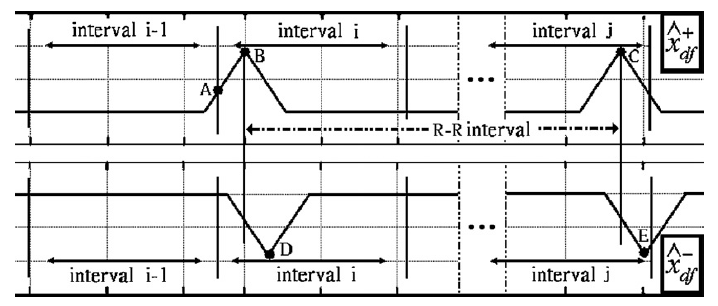
\includegraphics[width=1\textwidth]{dom6}
    \caption{Metoda selekcji ekstremów na podstawie odległości między nimi.}
 	 \label{fig:dom6}
\end{figure}
	
Detekcja załamków Q i S:
	
\begin{itemize}
	\item Zdefiniowanie pierwszego zakresu interwału, w którym wyszukiwane będą załamki Q i S. Jest to odcinek o długości 40 próbek (20 próbek przed wyznaczonym załamkiem R oraz 20 próbek za wyznaczonym załamkiem R). Dla obu części danego interwału wyznaczane są minimalne wartości i oznaczane odpowiednio jako $Q_1$ oraz $S_1$. 
	\item Detekcja załamków QRS kończy się na powyższym etapie w przypadku normalnego sygnału EKG. Jeżeli sygnał odbiega od standardowych zapisów EKG, potrzebne są dalsze kroki.
	\item Zdefiniowanie drugiego zakresu interwału, w którym wyszukiwane będą załamki Q i S. Drugi zakres jest dwukrotnym rozszerzeniem pierwszego zakresu w obu kierunkach (łączna długość 80 próbek dla częstotliwości próbkowania równej 360 Hz). Dla obu części danego interwału wyznaczane są minimalne wartości i oznaczane odpowiednio jako $Q_2$ oraz $S_2$.
	\item Następnie wyszukiwana jest pozycja załamka Q.
	\begin{itemize}
	\item Jeżeli pozycja $Q_1$ jest równa pozycji $Q_2$ to wtedy pozycja załamka Q równa się ich pozycji.
	\item Jeżeli prawdziwa jest poniższa nierówność (~\ref{eq:domE3}) to pozycja Q równa się pozycji $Q_2$

	\begin{equation} \label{eq:domE3}			
	 	MV_{QQ}>V_{Q1}+T_V
	\end{equation}			
			
Gdzie:
			
	\begin{itemize}
	\item $MV_{QQ}$ – maksimum w zakresie od $Q_1$ do $Q_2$
	\item $V_{Q1}$ – amplituda punktu $Q_1$
	\item $T_V$ – wartość progowa dobierana eksperymentalnie
	\end{itemize}
			
	\item Jeżeli prawdziwa jest poniższa nierówność (~\ref{eq:domE4}) to pozycja Q równa się pozycji $Q_1$
	
	\begin{equation} \label{eq:domE4}		
		V_{Q2}>V_{Q1}
	\end{equation}		
			
Gdzie:
			
	\begin{itemize}
		\item $V_{Q2}$ – amplituda punktu $Q_2$
	\end{itemize}			
			
	\item Jeżeli nie jest prawdziwa żadna z powyższych zależności to pozycja załamka Q jest równa pozycji punktu $Q_2$
\end{itemize}
	
Schemat detekcji załamka R znajduje się na rysunku ~\ref{fig:dom7}.	
	
	\item Detekcja załamka S
		
	\begin{itemize}
		
	\item Jeżeli pozycja $S_1$ jest równa pozycji $S_2$ to wtedy pozycja załamka S równa się ich pozycji.
	\item Jeżeli prawdziwa jest poniższa nierówność (~\ref{eq:domE5}) to pozycja S równa się pozycji $S_1$
		
	\begin{equation} \label{eq:domE5}
		V_{S2}>V_{S1}		
	\end{equation}
			
Gdzie:
			
	\begin{itemize}
		\item $V_{S1}$ – amplituda punktu $S_1$
		\item $V_{S2}$ – amplituda punktu $S_2$
	\end{itemize}
			
	\item Jeżeli nie jest prawdziwa żadna z powyższych zależności to pozycja załamka S jest równa pozycji punktu $S_2$
		
	\end{itemize}	
		
	\item Schemat detekcji załamków Q i S znajduje się na rysunku ~\ref{fig:dom8}.
		
	\begin{figure}
  		\centering
    	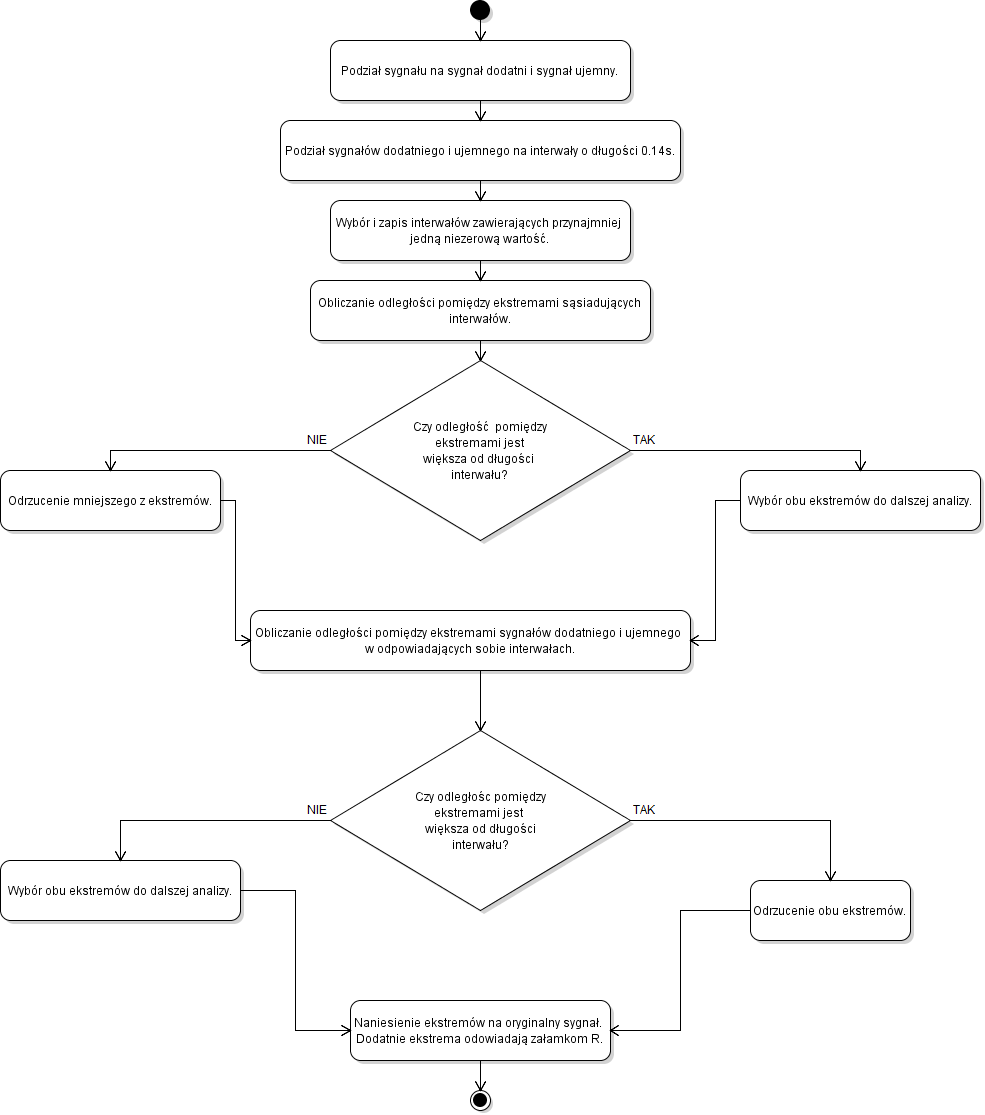
\includegraphics[width=1\textwidth]{dom7}
    	\caption{Schemat detekcji załamków R.}
 	 	\label{fig:dom7}
	\end{figure}
		
	\begin{figure}
  		\centering
    	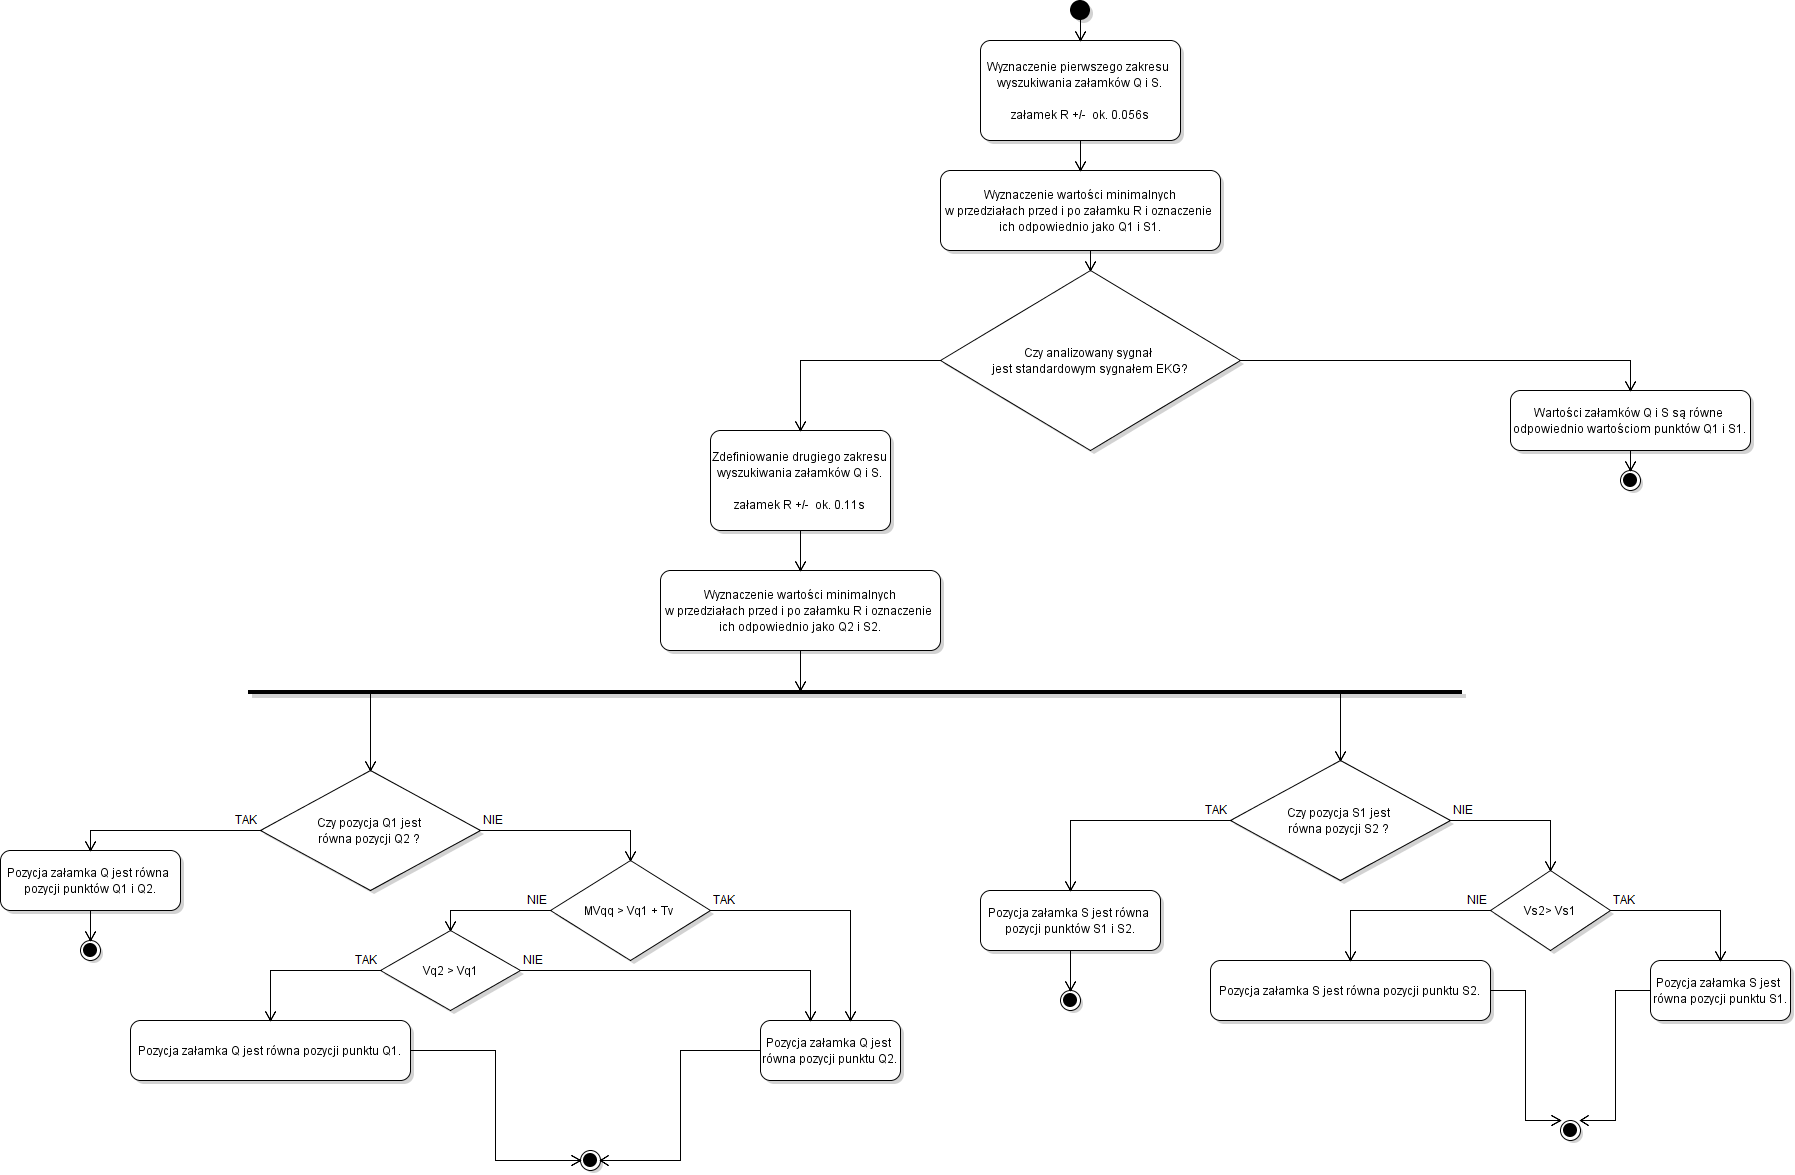
\includegraphics[width=1.2\textwidth, angle =90 ]{dom8}
    	\caption{Schemat detekcji załamków Q i S}
 	 	\label{fig:dom8}
	\end{figure}		
		
	\end{itemize}	
		

\subsection{Implementacja algorytmu w programie Matlab}

W pierwszej kolejności sygnał jest wczytywany (rysunek ~\ref{fig:dom9}). Następnie przeprowadzana jest filtracja typu notch (60Hz) oraz filtracja górnoprzepustowa (fc = 0,5Hz). Oba filtry zaprojektowano przy użyciu narzędzia fdatool, a następnie wyeksportowano otrzymane współczynniki i przeprowadzono filtrację. Ostatnim typem zastosowanej filtracji jest filtracja morfologiczna, która została zaimplementowana za pomocą funkcji imopen() oraz imclose(). Niestety nie udało się zaimplementować filtracji adaptacyjnej.  Wyniki wszystkich wyżej wymienionych filtracji są przedstawione na rysunkach ~\ref{fig:dom10},~\ref{fig:dom11},~\ref{fig:dom12}.

\begin{figure}
  	\centering
    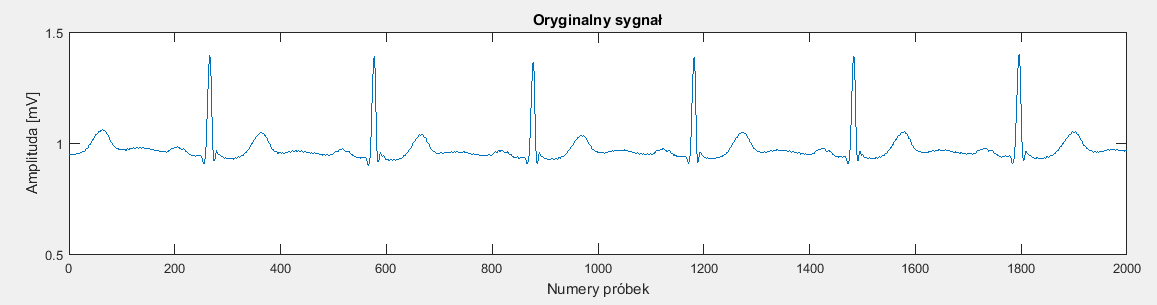
\includegraphics[width=1\textwidth]{dom9}
    \caption{Oryginalny sygnał EKG dla danych 103m.csv}
  	\label{fig:dom9}
\end{figure}

\begin{figure}
  	\centering
    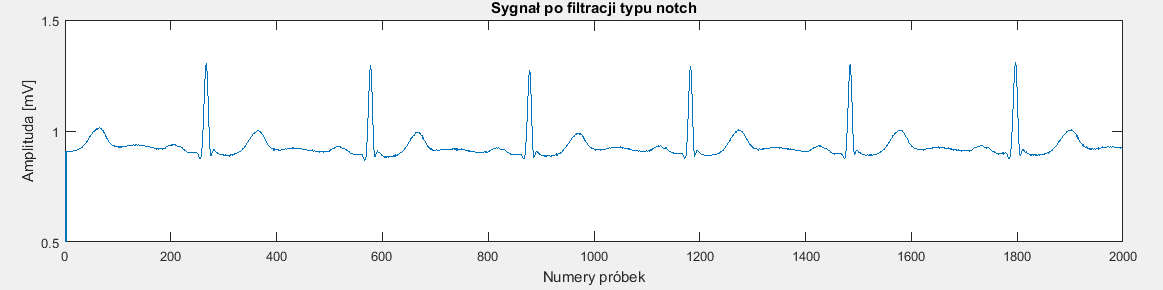
\includegraphics[width=1\textwidth]{dom10}
    \caption{Sygnał EKG po filtracji typu notch dla danych 103m.csv}
  	\label{fig:dom10}
\end{figure}

\begin{figure}
  	\centering
    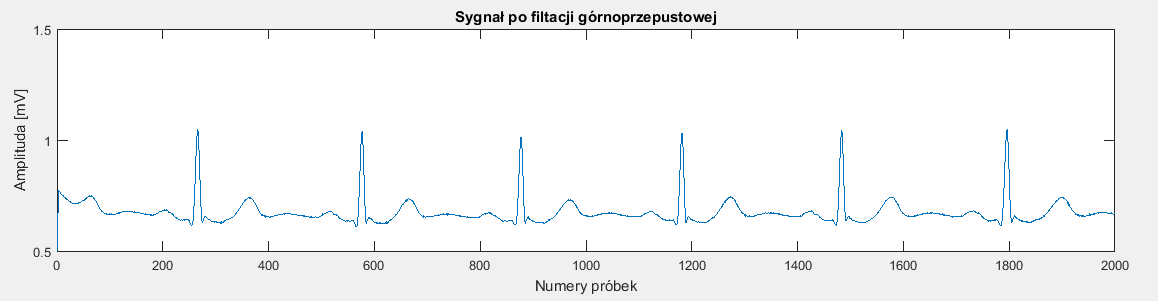
\includegraphics[width=1\textwidth]{dom11}
    \caption{Sygnał EKG po filtracji górnoprzepustowej dla danych 103m.csv}
  	\label{fig:dom11}
\end{figure}

\begin{figure}
  	\centering
    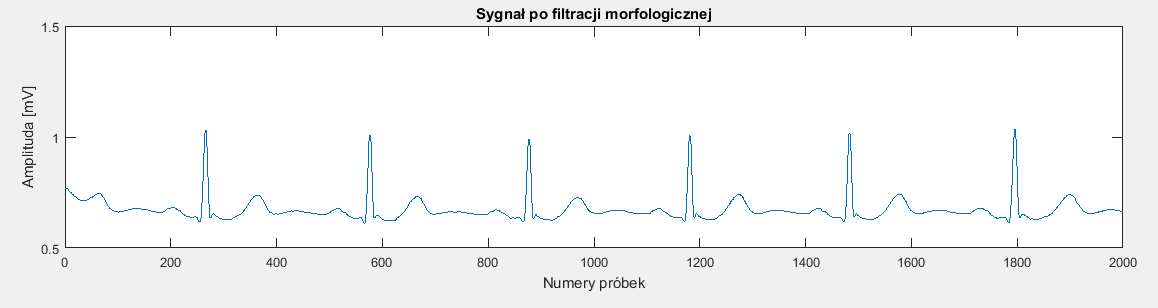
\includegraphics[width=1\textwidth]{dom12}
    \caption{Sygnał EKG po filtracji morfologicznej dla danych 103m.csv}
  	\label{fig:dom12}
\end{figure}

Następnie, przeprowadzane jest różnicowanie sygnału (rysunek ~\ref{fig:dom13}) oraz filtracja otrzymanego sygnału różnicowego za pomocą filtra dolnoprzepustowego (fc = 100Hz) (rysunek ~\ref{fig:dom14}). Ten filtr również został zaprojektowany przy użyciu narzędzia fdatool. Przed przystąpieniem do filtracji, na koniec sygnału różnicowego zostaje dodany wektor zer o długości odpowiadającej połowie liczby współczynników filtra. Dzięki temu likwidowane jest przesunięcie sygnału spowodowane filtracją.
 
\begin{figure}
  	\centering
    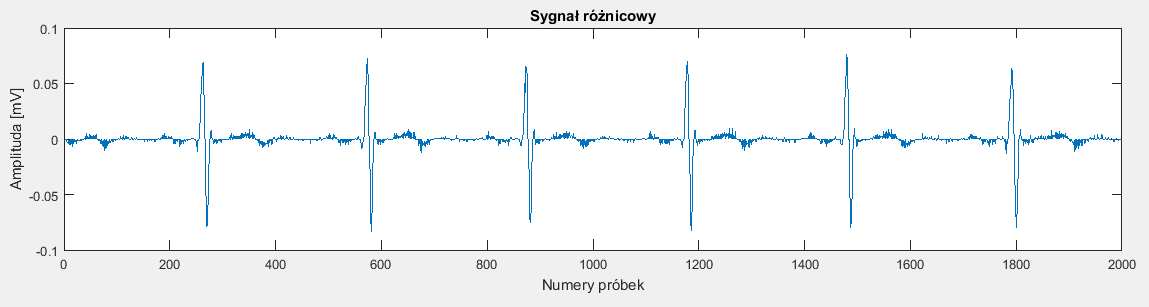
\includegraphics[width=1\textwidth]{dom13}
    \caption{Sygnał różnicowy dla danych 103m.csv}
  	\label{fig:dom13}
\end{figure}

\begin{figure}
  	\centering
    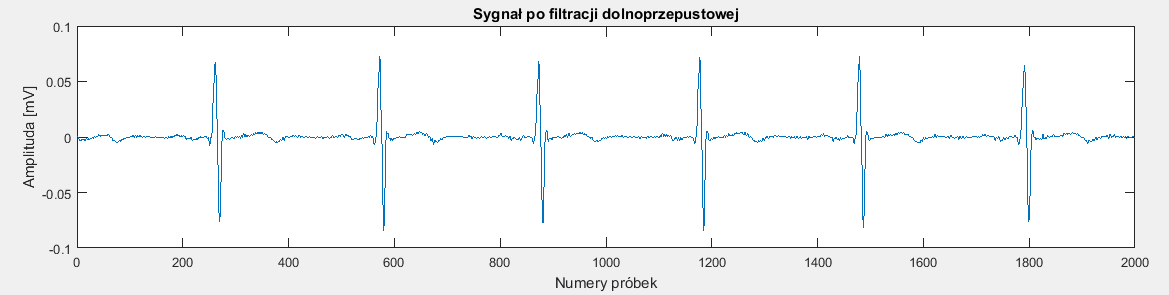
\includegraphics[width=1\textwidth]{dom14}
    \caption{Sygnał różnicowy po filtracji dolnoprzepustowej dla danych 103m.csv}
  	\label{fig:dom14}
\end{figure} 
 
Progowanie przefiltrowanego sygnału jest wykonywane z wykorzystaniem wartości MVP oraz MVN, wyliczonych na podstawie aktualnie analizowanego sygnału. Są to wartości średnie odpowiednio dodatnich oraz ujemnych amplitud w sygnale. Otrzymane wartości MVP oraz MVN są zwiększane czterokrotnie przed wykonaniem progowania. Wynik progowania jest przedstawiony na rysunku ~\ref{fig:dom15}. Po operacji progowania, następuje podział sygnału na dodatni i ujemny (rysunki ~\ref{fig:dom16} i ~\ref{fig:dom17}). 

\begin{figure}
  	\centering
    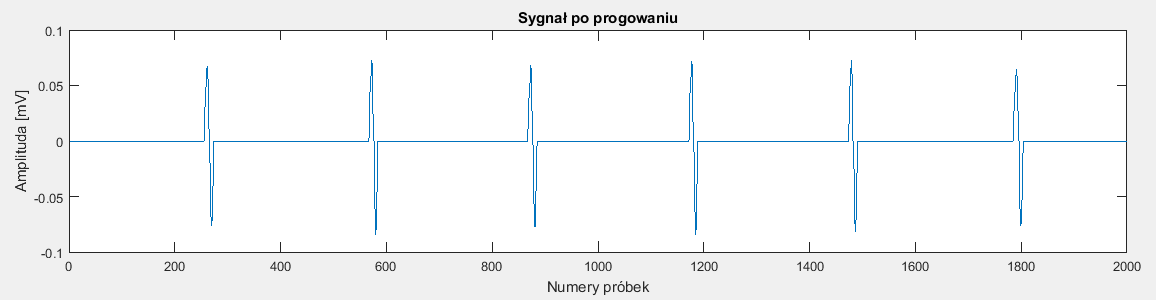
\includegraphics[width=1\textwidth]{dom15}
    \caption{Sygnał różnicowy po operacji progowania dla danych 103m.csv}
  	\label{fig:dom15}
\end{figure} 

\begin{figure}
  	\centering
    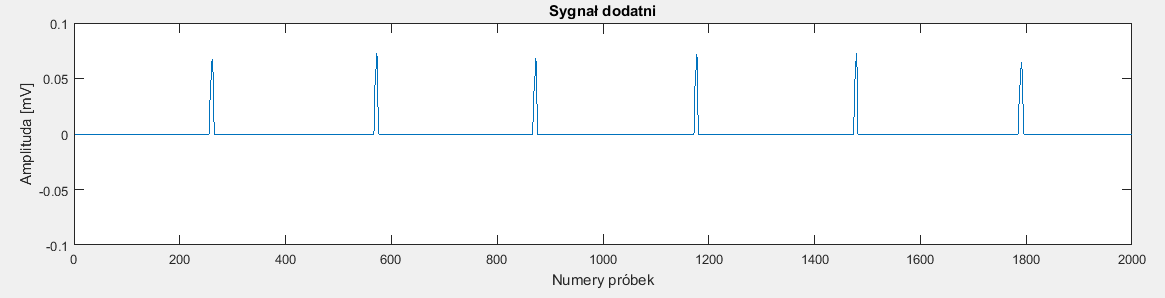
\includegraphics[width=1\textwidth]{dom16}
    \caption{Sygnał dodatni dla danych 103m.csv}
  	\label{fig:dom16}
\end{figure} 

\begin{figure}
  	\centering
    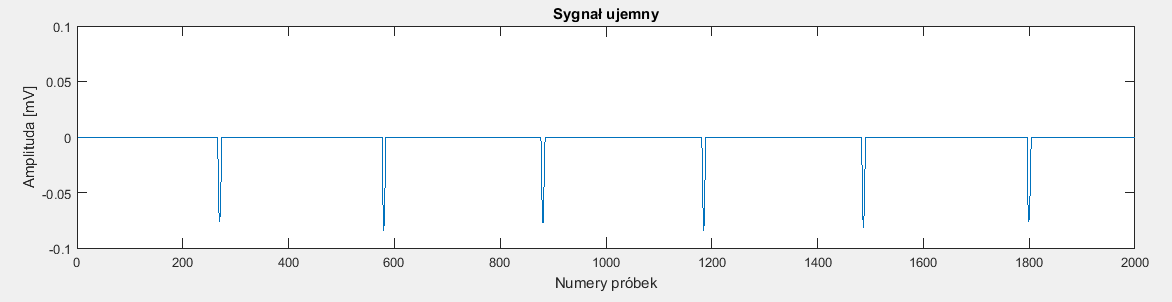
\includegraphics[width=1\textwidth]{dom17}
    \caption{Sygnał ujemny dla danych 103m.csv}
  	\label{fig:dom17}
\end{figure}

Dalszym krokiem jest podział sygnałów (zarówno ujemnego jak i dodatniego) na interwały o długości 50 próbek i wykrycie odpowiednio najmniejszej oraz największej wartości w interwale. Jeżeli wartości maksymalne i minimalne otrzymane w interwałach są różne od zera, to do wektorów zapisywane są numery próbek odpowiadające danym ekstremom. Otrzymane numery próbek odpowiadające maksimom i minimom w odpowiednich interwałach są wykorzystywane do dalszej analizy. 

Analogiczne operacje zostają przeprowadzone dla sygnał dodatniego oraz ujemnego. W przypadku sygnału dodatniego, tworzony jest nowy wektor. W pierwszej kolejności, obliczana jest odległość między pierwszą i drugą próbką sygnału dodatniego. Jeżeli odległość jest większa od 50, to obie próbki są zapisywane w wektorze. Jeżeli odległość jest mniejsza od zera, to zapisywana jest próbka, dla której wartość amplitudy jest większa. 

Następnie porównywane są ostatnie próbki nowego wektora z kolejnymi próbkami sygnału dodatniego. Jeżeli odległość między analizowanymi próbkami jest większa, to bieżąca próbka jest wpisywana na końcu wektora. Jeżeli wartość bieżącej próbki jest większa od wartości ostatniej próbki sygnału dodatniego, to próbka bieżąca jest wpisywana na miejsce ostatniej próbki. Wyniki powyższej operacji są zapisywane jako wykryte załamki R (rysunek ~\ref{fig:dom18}).

\begin{figure}
  	\centering
    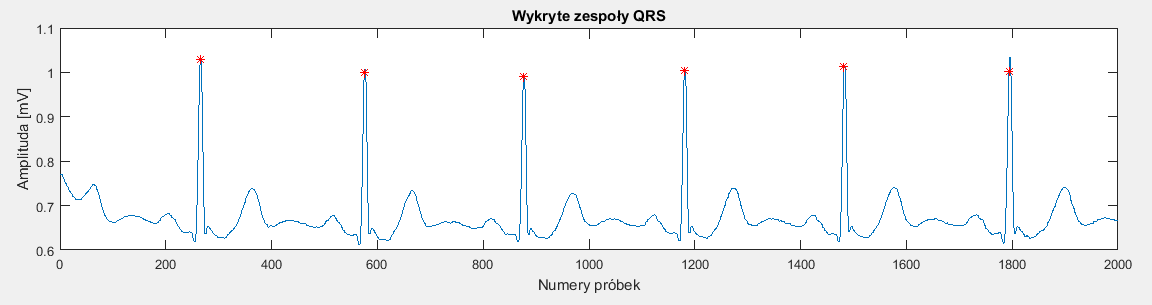
\includegraphics[width=1\textwidth]{dom18}
    \caption{Sygnał EKG z zaznaczonymi załamkami R dla danych 103m.csv}
  	\label{fig:dom18}
\end{figure}

Ostatnim etapem jest detekcja załamków Q oraz S. W tym celu, wyznaczane są interwały obejmujące: załamek R oraz 20 wcześniejszych próbek, załamek R oraz 20 późniejszych próbek. Następnie, w pierwszym zakresie obliczane jest minimum, które odpowiada załamkowi Q. W drugim zakresie obliczane jest minimum, które odpowiada załamkowi S.

\subsection{Implementacja algorytmu w języku C++}

W przypadku implementacji algorytmu w C++, nie udało się przeprowadzić filtracji sygnału. Wczytany sygnał zostaje poddany operacji różnicowania oraz progowania, a następnie podzielony na sygnał dodatni i ujemny. Dalszym krokiem jest wykrycie maksimów i minimów w interwałach o długości 50 próbek oraz porównywanie otrzymanych wyników, analogicznie jak w przypadku prototypu w środowisku MATLAB. Z powodu braku filtracji, na końcu algorytmu zaimplementowano dodatkowe progowanie otrzymanych maksimów. Wartość progu wynosi 50\% wartości największego maksimum. Wykryte numery próbek są zapisywane jako wykryte załamki R. Dodatkowo, algorytm zawiera operację detekcji załamków Q i S analogiczną do tej zaimplementowanej w środowisku MATLAB.

\subsection{Podsumowanie}

Algorytm Difference Operation Method jest prostą, niewymagającą skomplikowanych przekształceń matematycznych, metodą detekcji załamków QRS. Metoda ta pozwala na szybką detekcję, ze względu na niską złożoność obliczeniową. Wyznaczone parametry czułości, precyzji i skuteczności detekcji dla sygnałów pochodzących z MIT-BIH arrhythmia database, pozwalają stwierdzić, że metoda ta daje zadowalające rezultaty dla większości przypadków. Algorytm nie sprawdza się niestety dla niestandardowych sygnałów EKG, co objawia się niską wartością wyżej wspomnianych parametrów. Algorytm DOM odznacza się dużą dokładnością detekcji. Dla większości sygnałów, precyzja detekcji wynosi 100 procent.

\newpage

\begin{thebibliography}{9}
 
\bibitem{domB1} 
Yun-Chi Yeha, Wen-June Wanga 
\textit{QRS complexes detection for ECG signal: The Difference Operation Method.}. 
Computer methods and programs in biomedicine, 2008, nr 91 s. 245-254.

\end{thebibliography}

\newpage

\section{Empirical Mode Decomposition}
	Algorytm EMD polega na rozłożeniu sygnału na skończoną ilość tzw. istotnych funkcji składowych $c_j$(IFM ang.Intrinsic Mode Functions), które wynikają z cech sygnału a nie funkcji bazowej (jak w przypadku transformacji Fouriera czy Falkowej).

Warto wspomnieć o tym, iż w przeciwieństwie do transformacji falkowej, podczas
empirycznej dekompozycji modalnej nie następuje przeciekanie energii w pobliżu
częstotliwości, które są analizowane. Natomiast głównym minusem tej metody jest
zauważalna niedokładność przy niskich częstotliwościach sygnału \cite{dwa}.

 \vspace{1em} 

Każda funkcja $c_j$ to jedna prosta postać sygnału drgań, która zapewnia następujące warunki:

\vspace{2em}

(a) Zbiór wartości IMF zawiera taką samą liczbę ekstremów i miejsc zerowych lub liczba ta
może różnić się najwyżej o jedno miejsce zerowe

 \vspace{1em} 

(b) Średnia wartość obwiedni określona przez lokalne minima i maksima w każdym
punkcie IMF jest równa zero

\vspace{2em}

Weźmy pod uwagę sygnał \textit{s(t)}. Empiryczną dekompozycję modalną można przedstawić w
następujących krokach \cite{dwa} \cite{trzy} \cite{cztery}:

 \vspace{1em} 
 
(1) Wyznaczenie lokalnych minimów i maksimów analizowanego sygnału \textit{s(t)}

(2) Połączenie lokalnych maksimów krzywą trzeciego stopnia – utworzenie górnej
obwiedni sygnału – \textit{EnvMax(t)}

(3) Połączenie lokalnych minimów krzywą trzeciego stopnia – utworzenie dolnej obwiedni
sygnału – \textit{EnvMin(t)}

(4) Obliczenie wartości średniej górnej i dolnej obwiedni w każdym punkcie sygnału
dyskretnego(\ref{w1}):

 \vspace{1em} 
 
\begin{equation}
m_1(t) = \frac{1}{2}(EnvMax(t) + EnvMin(t))
\label{w1}
\end{equation}

(5) Obliczenie odchylenia wartości w każdym punkcie sygnału od wartości średniej(\ref{w2}):

\begin{equation}
h_1(t) = (s(t) - m_1(t))
\label{w2}
\end{equation}

W tym momencie następuje sprawdzenie czy $h_1$(t) spełnia warunki wspomniane powyżej
(punkty (a) i (b).

\vspace{0.5em}

Jeśli:

\vspace{0.5em}

- TAK - wyrażenie to można uznać za istotną funkcję składową $c_1$

- NIE - wyrażenie $h_1$(t) traktuje się, jako sygnał oryginalny i powtarza obliczenia z punktów (1) -(5) do momentu uzyskania istotnej funkcji składowej $c_j$

(6) Obliczenie składowej reszty $r_1$(t) poprzez usunięcie pierwszej istotnej funkcji
składowej z sygnału pierwotnego \textit{s(t)} (\ref{w3}):
\begin{equation}
r_1(t) = (s(t) - h_1(t))
\label{w3}
\end{equation}

(7) Po wyliczeniu w punktach (1) - (5) drugiej IMF, powtórzenie obliczeń traktując sygnał
reszty $r_1$(t) z poprzedniej iteracji, jako sygnał oryginalny (\ref{w4}):
\begin{equation}
r_2(t) = (r_1(t) - h_2(t))
\label{w4}
\end{equation}

(8) Powtórzenie obliczeń dla n-kolejnych razy (\ref{w5}):
\begin{equation}
r_n(t) = (r_{n-1}(t) - h_n(t))
\label{w5}
\end{equation}

(9) Obliczenie kryterium zatrzymania procesu – dekompozycja może zostać zatrzymana,
kiedy kolejne $r_n$(t) stają się monotonicznymi funkcjami nie wnoszącymi istotnych
informacji. Popularnym kryterium zatrzymania jest tzw. NSD (ang. Normalized
Standard Difference), określany wzorem (\ref{w6}):
\begin{equation}
NSD=\sum_{t=1}^{T} \frac{|h_{n-1}(t)-h_n(t)|^2}{{h^2}_n(t)}
\label{w6}
\end{equation}

(10) Ostatecznie, sygnał wejściowy może zostać zapisany w postaci sum istotnych
funkcji składowych z sygnałami reszt (\ref{w7}):
\begin{equation}
\label{w7}
s(t)=sum_{n=1}^{N} h_n(t)+ r_n 
\end{equation}

\subsection{Koncepcja proponowanego rozwiązania}

Opisana wcześniej Empiryczna Dekompozycja Modalna jest popularna podczas przetwarzania
sygnałów biomedycznych, w tym także podczas detekcji zespołów QRS. Jednak proces
wykrywania załamków obejmuje szerszy zakres, w skład, którego wchodzą m.in. filtracja
górno- i dolnoprzepustowa czy transformacja nieliniowa. Dokładny przebieg tego procesu
został pokazany na schemacie poniżej (Rys. \ref{proces})\cite{trzy}.


\begin{figure}
\label{proces}
	\centerline{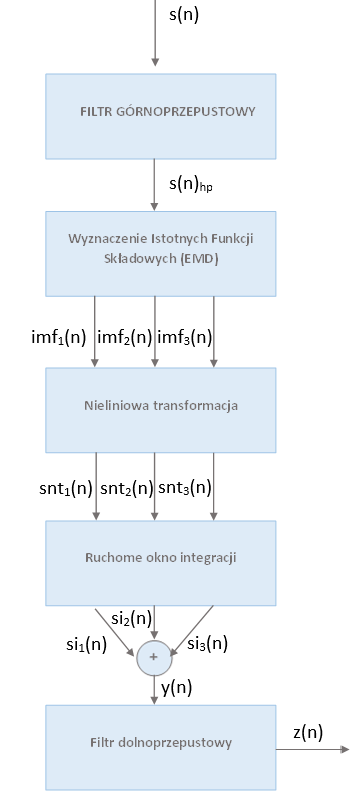
\includegraphics[scale=0.9]{proces}}
	\caption{Kroki, jakie podjęto w celu detekcji załamków QRS za pomocą metody EMD.}
\end{figure}
\FloatBarrier


\subsection{Prototyp rozwiązania w środowisku MATLAB}

Stworzenie prototypu w środowisku MATLAB obejmuje wykorzystanie algorytmu postępowania
przedstawionego na rysunku \ref{proces}. W dalszej części projektu zostaną przedstawione poszczególne kroki wyżej opisanego algorytmu, które stanowiły punkt wyjścia do implementacji w C++.

\vspace{1em}

a) Filtracja górnoprzepustowa

Pierwszy z zastosowanych kroków pozwolił na usunięcie z sygnału częstotliwości z
zakresu 0-1 Hz, które miały znaczny wpływ na pływającą linię izoelektryczną. Biorąc
pod uwagę wiedzę nabytą podczas laboratorium, zdecydowano się na filtr Butterwortha V rzędu
o częstotliwości odcięcia 1Hz.

\vspace{1em}

Wyniki filtracji, wraz z usuniętym szumem przedstawiono na Rys. \ref{filtracja}

\vspace{1em}

\begin{figure}[h!]
\label{filtracja}
	\centerline{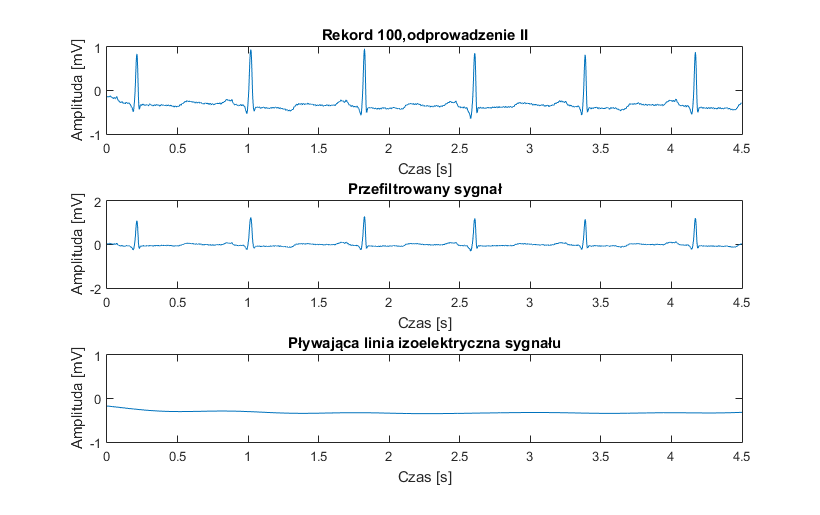
\includegraphics[scale=0.9]{pierwszy}}
	\caption{Wyniki filtracji górnoprzepustowej}
\end{figure}
\FloatBarrier

\vspace{1em}

b) Empiryczna Dekompozycja Modalna

Następnie została wykonana EMD, która szczegółowo została opisana w poprzednim podrozdziale
niniejszego raportu. Rys.\ref{emd} przedstawia 3 pierwsze istotne funkcje składowe IMF.

\vspace{1em}

\begin{figure}[h!]
\label{emd}
	\centerline{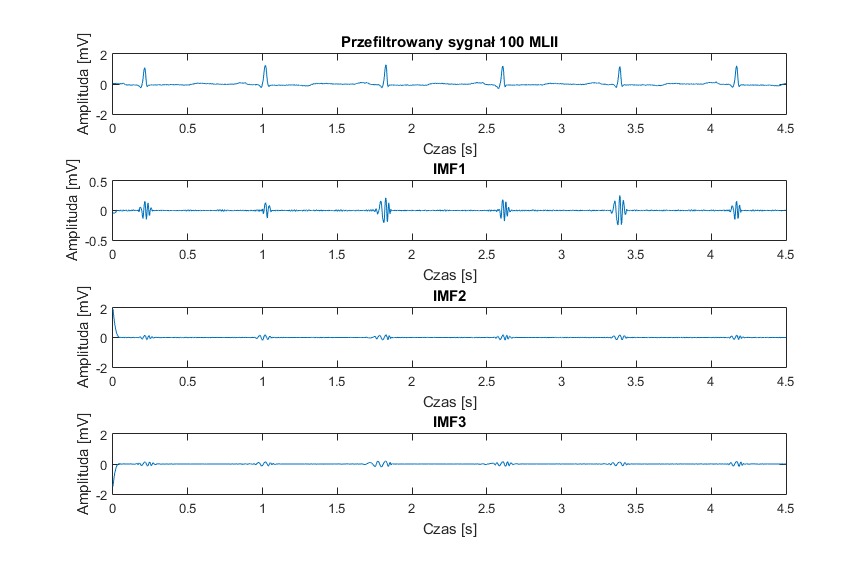
\includegraphics[width=\textwidth]{drugi}}
	\caption{Oryginalny przefiltrowany sygnał i jego trzy istotne funkcje składowe}
\end{figure}
\FloatBarrier

 \vspace{1em}

c) Transformacja nieliniowa

Po dokonaniu estymacji IMF, kolejnym krokiem była transformacja nieliniowa
wyznaczona z wzoru \cite{trzy}:

\begin{equation}
\label{w9}
y(n) = abs(x(n) \cdot x(n - 1) \cdot x(n - 2))
\end{equation}
\begin{center}

dla x(n), x(n-1), x(n-2) tego samego znaku

\end{center}

\begin{equation}
y(n) = 0 
\label{w9}
\end{equation}

\begin{center}
w przeciwnym wypadku
\end{center}

\vspace{1em}

gdzie:

x(n) = $imf_n$(k)
y(n) = $snt_k$(n)


 \vspace{1em}

d) Ruchome okno integracji

W celu integracji wszystkich sygnałów konieczne było zastosowanie ruchomego
okna integracji, które jest przedstawione poniższym wzorem (\ref{w9}):
\begin{equation}
\label{w10}
si_k(n)=(\frac{1}{M})(snt_k(n-(M-1)) + snt_k(n-(M-2)) + \ldots + snt_k(n))
\end{equation}

Gdzie M to liczba próbek w oknie integracji.


e) Filtracja dolnoprzepustowa

Aby usunąć końcowe zakłócenie został zastosowany dolnoprzepustowy filtr
Butterwortha pierwszego rzędu.

 \vspace{1em}
 
Na rysunku \ref{butter} pokazano wyniki transformacji nieliniowej i integracji oraz filtracji dolnoprzepustowej.

\begin{figure}[h!]
\label{butter}
	\centerline{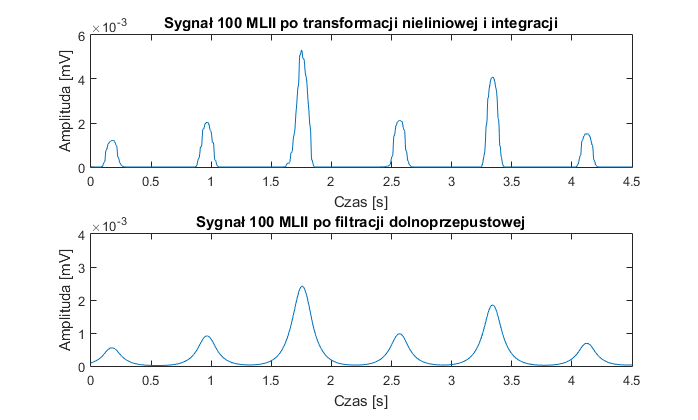
\includegraphics[width=\textwidth]{trzeci}}
	\caption{Transformacja i integracja nieliniowa sygnału, przed oraz po filtracji dolnoprzepustowej}
\end{figure}
\FloatBarrier

 \vspace{1em}
 \newpage
 Ostatnim krokiem w przedstawionym algorytmie było znalezienie szczytów za pomocą funkcji findpeaks().
 Wyniki detekcji załamka QRS za pomocą Empirycznej Dekompozycji Modalnej przedstawiono na rysunku \ref{ostatni}.

\begin{figure}[h!]
\label{ostatni}
	\centerline{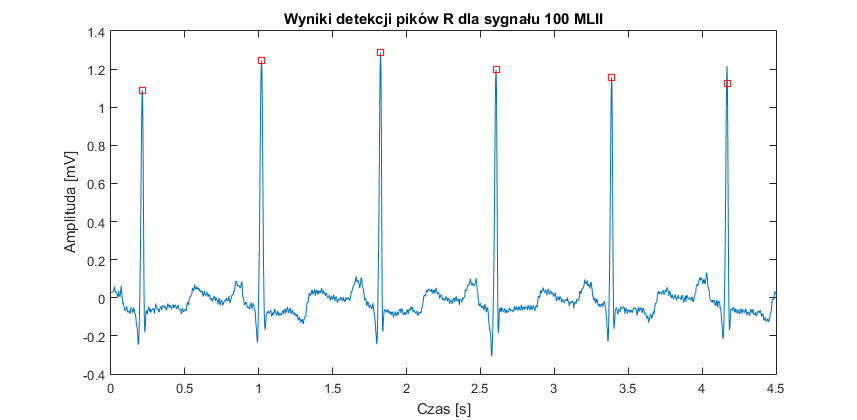
\includegraphics[width=\textwidth]{czwarty}}
	\caption{Wyniki detekcji załamka QRS za pomocą Empirycznej Dekompozycji Modalnej}
\end{figure}


\clearpage

\begin{thebibliography}{9}

 
\bibitem{jeden}
Huang N.E, Shen Z., Long S.R., Wu M.C., Shih H.H., Zheng Q., Yen N., Tung C.C., Liu
H.H.: \textit{“The empirical mode decomposition and the Hilbert spectrum for nonlinear and
non-stationary time series analysis” }. Proceedings of the Royal Society of London A:
Mathematical, Physical and Engineering Sciences, 1998, vol. 454, no. 1971, pp.
903-995.

 \vspace{0.5em}
 
\bibitem{dwa}
Zachwieja J.: \textit{“Wyważanie wirnika wentylatora promiennego w różnych stanach
dynamicznych”.} Rozprawy. Uniwersytet Technologiczno - Przyrodniczy w Bydgoszczy,
2012, 153.

\vspace{0.5em}

\bibitem{trzy}
Slimane H., Nait-Ali A.: \textit{“QRS complex detection using Empirical Mode Decomposition”.}
Digital Signal Processing, 2010, 20(4), pp. 1221-1228.

\vspace{0.5em}

\bibitem{cztery}
Pal S., Mitra M.: \textit{“Empirical mode decomposition based ECG enhancement and QRS
detection”.} Computers in biology and medicine, 2012, 42(1),pp. 83-2.

\end{thebibliography}

\newpage
\section{Detekcja QRS z użyciem filtracji kwadratowej}
\bigskip
Algorytmy mające na celu wyznaczenie zespołów QRS składają się z dwóch części: przetwarzania wstępnego oraz części detekcyjnej. Algorytm opisany poniżej jest rozwiązaniem zaproponowanym przez dr Pornchai Phukpattaranont~\cite{QF article}. Sygnał EKG zostaje w pierwszej kolejności przefiltrowany z użyciem filtru kwadratowego. Zastosowanie tego typu rozwiązania pozwala na zwiększenie stosunku sygnału do szumu. Dzięki temu odpowiednia wydajność detekcji może być uzyskana bez potrzeby użycia progowania adaptacyjnego oraz postprocessingu.

Opisane rozwiązanie składa się zatem z części odpowiedzialnej za projektowanie filtru oraz części mającej na celu wyznaczenie zespołów QRS. Szczegółowy opis wspomnianych etapów został zawarty w rozdziałach poniżej.
\bigskip
\subsection{Opis teoretyczny}
\bigskip
\subsubsection{Filtracja}
\bigskip
W przeciwieństwie do filtrów liniowych, filtry kwadratowe mają tę zaletę, iż posiadają różne stopnie swobody do optymalizacji procesu usuwania szumu z~sygnału EKG.

Filtr kwadratowy o liniowej fazie został zaprojektowany na podstawie sumy dwóch dwuwymiarowych filtrów Gaussa. W ogólności, odpowiedź częstotliwościowa filtru QF (ang. Quadratic Filter), na podstawie dyskretnej transformaty Fouriera, może zostać wyrażona wzorem:
\medskip
\begin{equation}
\label{QF1}
H(e^{j\omega_{1k}},e^{j\omega_{2l}})=\sum_{n_1=0}^{N_1-1}\sum_{n_2=0}^{N_2-1}h(n_1,n_2)e^{-jn_1\omega_{1k}}e^{-jn_2\omega_{2l}}
\end{equation}
\medskip
Gdzie H jest dwuwymiarową odpowiedzią częstotliwościową filtru QF, h to współczynniki filtru, \begin{math}N_{1}\end{math} oraz \begin{math}N_{2}\end{math} to długość filtru odpowiednio dla \begin{math}n_{1}\end{math} oraz \begin{math}n_{2}\end{math}. Celem projektowania filtru jest wyznaczenie współczynników GF, \begin{math}h(n_{1},n_{2})\end{math}.

Zadanie to można wypełnić biorąc pod uwagę, iż odpowiedź częstotliwościowa dana jest także wzorem:
\medskip
\begin{equation}
\label{QF2}
H(e^{j\omega-{1k}},e^{j\omega-{2l}})=G(\omega_{1k},\omega_{2l})e^{j\phi(\omega_{1k},\omega_{2l})}
\end{equation}
\medskip

Gdzie \begin{math}G(\omega_{1k},\omega_{2l})\end{math} reprezentuje żądany moduł, natomiast \begin{math}\phi(\omega_{1k},\omega_{2l})\end{math} - fazę. Widmo fazowe dane jest wzorem:
\medskip
\begin{equation}
\label{QF3 - widmo fazowe}
\phi(\omega_{1k},\omega_{2l})=-\frac{N_1-1}{2}\omega_{1k}-\frac{N_2-1}{2}\omega_{2l}
\end{equation}
\medskip

Gdzie \begin{math}\omega_{1k}=(\frac{2\pi k}{M_1})-\pi, k=0,1,...,M_1-1\end{math} a \begin{math}\omega_{2l}=(\frac{2\pi l}{M_2})-\pi, l=0,1,...,M_2-1\end{math}. Użyto filtru o rozmiarze \begin{math}N_1=N_2=N=37\end{math}. W rezultacie opóźnienie fazowe sygnału wyjściowego jest równe (N-1)/2.

Zaproponowano filtr QF oparty o sumę dwóch dwuwymiarowych filtrów Gaussa. Zależność tę zobrazować można w następujący sposób:
\medskip
\begin{equation}
\label{QF4 - suma dwoch filtrow}
G(\omega_{1k},\omega_{2l})=\frac{G_1(\omega_{1k},\omega_{2l})+G_2(\omega_{1k},\omega_{2l})}{max\{G_1+G_2\}}
\end{equation}
\medskip

Gdzie
\medskip
\begin{equation}
\label{QF5 - Gi}
G_i(\omega_{1k},\omega_{2l})=exp\{-[A(\omega_{1k}-\omega_{ai})^2+B(\omega_{1k}-\omega_{ai})(\omega_{2l}-\omega_{bi})+C(\omega_{2l}-\omega_{bi})^2]\}
\end{equation}
\medskip

Dla i=1,2. Parametry A, B oraz C:
\medskip
\begin{equation}
\label{QF6  - A}
A=(\frac{cos\theta}{\sigma_x})^2+(\frac{sin\theta}{\sigma_y})^2
\end{equation}

\begin{equation}
\label{QF7  - B}
B=-\frac{sin2\theta}{\sigma_x^2}+\frac{sin2\theta}{\sigma_y^2}
\end{equation}

\begin{equation}
\label{QF8  - C}
C=(\frac{sin\theta}{\sigma_x})^2+(\frac{cos\theta}{\sigma_y})^2
\end{equation}
\medskip

Współczynniki \begin{math}(\omega_{ai},\omega_{bi})\end{math} są środkami filtrów Gaussa, \begin{math}\sigma_x \end{math} oraz \begin{math} \sigma_y \end{math} to stałe definiujące szerokość przepustowości wzdłuż dwóch kierunków, natomiast \begin{math}\theta\end{math} to kąt obrotu. Przyjęto następujące wartości: centra \begin{math}(\omega_{ai},\omega_{bi})\end{math} w punktach (-0.7,0.7) oraz (0.7, -0.7), \begin{math}\sigma_x = 0.3\end{math}, \begin{math}\sigma_y = 0.2\end{math}, \begin{math}\theta = -\pi / 4\end{math}.

Po otrzymaniu odpowiedzi w dziedzinie częstotliwościowej ze wzoru \ref{QF2}, współczynniki filtru \begin{math}h(n_1,n_2)\end{math} można otrzymać poprzez zastosowanie odwrotnej dyskretnej transformaty Fouriera, korzystając ze wzoru \ref{QF9}.
\medskip
\begin{equation}
\label{QF9}
h(n_1,n_2)=\frac{1}{M_1M_2}\sum_{k=0}^{M_1-1}\sum_{l=0}^{M_2-1}H(e^{j\omega_{1k}},e^{j\omega_{2l}})e^{jn_1\omega_{1k}}e^{jn_2\omega_{2l}}
\end{equation}
\medskip

gdzie \begin{math}M_1\end{math} oraz  \begin{math}M_2\end{math} to ilość punktów użytych w odwrotnej transformacji, odpowiednio wzdłuż \begin{math}\omega_{1k}\end{math}  oraz \begin{math}\omega_{2l}\end{math}.

Sygnał EKG po operacji usuwania szumów, a zatem po przefiltrowaniu, wyrażony jest wzorem \ref{QF10}.
\medskip
\begin{equation}
\label{QF10}
y[n]= \sum_{k_1=0}^{P-1}\sum_{k_2=0}^{P-1}h[k_1,k_2]x[n-k_1]x[n-k_2]
\end{equation}
\bigskip

\subsubsection{Detekcja zespołów QRS}
\bigskip

Szumy w sygnale wejściowym x[n] zostają ograniczone poprzez użycie zaprojektowanego filtru QF. Po tej operacji, z otrzymanego sygnału y[n] zostaje wyznaczona obwiednia z[n]. Następnie, zdefiniowana zostaje wartość progowa, w celu wyznaczenia interwału czasowego [t1 t2], w którym znajduje się zespół QRS. Ostatecznie miejsce, w którym występuje załamek R zostaje zlokalizowane poprzez odnalezienie czasu tR, dla którego amplituda sygnału osiąga maksimum.

W sposób szczegółowy algorytm ten można opisać w następujących krokach:
\begin{enumerate}
\item Wyznaczenie sygnału y[n] z wejściowego sygnału EKG x[n] poprzez przetworzenie go filtrem QF.
\item wyznaczenie obwiedni z[n] z sygnału y[n] przy użyciu filtru wyszukującego maksimum, danego wzorem:
\begin{equation}
\label{QF11 - obwiednia}
z[n]= \max_{k\in [n-L+1,n]}y[k]
\end{equation}
\item Detekcja załamka R w zespole QRS za pomocą następujących kroków:
\begin{itemize}
\item Wyliczenie wartości progowej thv z zależności \begin{math}thv=\lambda y_m[n]\end{math}, gdzie \begin{math}y_m[n]\end{math} to wartość maksymalna sygnału y[n], a  \begin{math}\lambda\end{math} to wartość stała z~przedziału od 0,10 do 0,17.
\item Znalezienie przedziałów czasowych, w których sygnał z[n] jest większy od wartości progowej thv oraz wyznaczenie dla nich czasu początkowego t1, czasu połówkowego th, oraz czasu kończącego t2.
\item Wyznaczenie amplitudy sygnału y[n] dla th. Jeśli amplituda jest większa od zera, co oznacza, że nie jest to przedwczesny skurcz komorowy, należy przejść do kolejnego podpkt, w przeciwnym przypadku do ostatniego.
\item Wyznaczenie lokalizacji załamka R z przedziału czasowego [t1 t2], w~miejscu gdzie sygnał osiąga maksimum.
\item Wyznaczenie lokalizacji załamka R z przedziału czasowego [t1 th], w~miejscu gdzie sygnał osiąga maksimum.
\end{itemize}
\end{enumerate}

\newpage
\subsection{Implementacja w środowisku Matlab}
\bigskip

W środowisku programistycznym Matlab zaimplementowano prototyp algorytmu służącego do detekcji QRS z użyciem filtracji kwadratowej. Program składał się z następujących części:
\begin{enumerate}
\item Projektowanie dwuwymiarowego filtru kwadratowego - wyznaczenie współczynników.
\item Filtracja sygnału z użyciem zaprojektowanego filtru.
\item Wyznaczanie progu na podstawie maksimum przefiltrowanego sygnału.
\item Wyliczanie obwiedni przefiltrowanego sygnału.
\item Progowanie obwiedni sygnału . Wyznaczanie czasów początkowych, końcowych oraz połówkowych.
\item Odnajdywanie maksimów sygnału w zadanych przedziałach czasowych.
\end{enumerate}

Pierwszym etapem było wyznaczenie współczynników dwuwymiarowego filtru kwadratowego opartego na dwóch filtrach Gaussa. Przyjęto następujące wartości: rozmiar filtru \begin{math}N=M=37\end{math}, centra \begin{math}(\omega_{ai},\omega_{bi})\end{math} w punktach (-0.7,0.7) oraz (0.7, -0.7), \begin{math}\sigma_x = 0.3\end{math}, \begin{math}\sigma_y = 0.2\end{math}, \begin{math}\theta = -\pi / 4\end{math}. Na podstawie wzorów \ref{QF6  - A}, \ref{QF7  - B} oraz \ref{QF8  - C} obliczono stałe parametry A, B oraz C. Następnie, przy użyciu zagnieżdżonych pętli for obliczono moduły oraz fazę dla dwóch filtrów Gaussa - \begin{math} G_1, G_2, O\end{math}. Zsumowano oraz znormalizowano wartości połączonych filtrów, a w dalszej kolejności obliczono odpowiedź częstotliwościową H. Na podstawie wzoru \ref{QF9}, określającego odwrotną transformację Fouriera, otrzymano wartości współczynników żądanego filtra - \begin{math} h(n_1,n_2)\end{math}.

Kolejnym etapem była filtracja sygnału z użyciem wyznaczonych współczynników.Zrealizowano to zadanie poprzez użycie trzech zagnieżdżonych pętli for otrzymując w efekcie przefiltrowany sygnał y[n]. Następnie wyznaczono próg jako iloczyn wartości maksymalnej w sygnale y[n] oraz parametru \begin{math}\lambda\end{math}. Wartość tego parametru przyjęto na poziomie 0.1.

Następnym krokiem realizowanym w programie było wyznaczenie obwiedni sygnału. Dokonano tego na podstawie wzoru \ref{QF11 - obwiednia}, stosując funkcję odnajdującą maksimum w zadanym oknie. Zgodnie ze szczegółowym opisem zamieszczonym powyżej,w dalszym etapie wyznaczono czasy początkowe oraz końcowe, jako miejsca, w których sygnał obwiedni zmienia wartości z mniejszej od progu na większą i odwrotnie. Na tej podstawie obliczono czasy połówkowe otrzymanych przedziałów czasowych.

Ostatnim krokiem było wyznaczenie maksimów w odpowiednio dobranych przedziałach czasowych. Maksima odnalezione w sygnale przefiltrowanym sprawdzano w odniesieniu do sygnału początkowego, otrzymując wartości ostateczne. Miejsca, w których oznaczono wartości maksymalne są miejscami, w których wykryto załamek R.

\newpage
Działanie omawianego algorytmu na przykładowym sygnale zostało przedstawione na Rys.\ref{QF rys1}. Górna ilustracja przedstawia fragment oryginalnego sygnału, środkowa tenże fragment po filtracji, natomiast dolna - obwiednię sygnału wraz z wyznaczonym progiem.

\medskip
\begin{figure}[h]
\centering
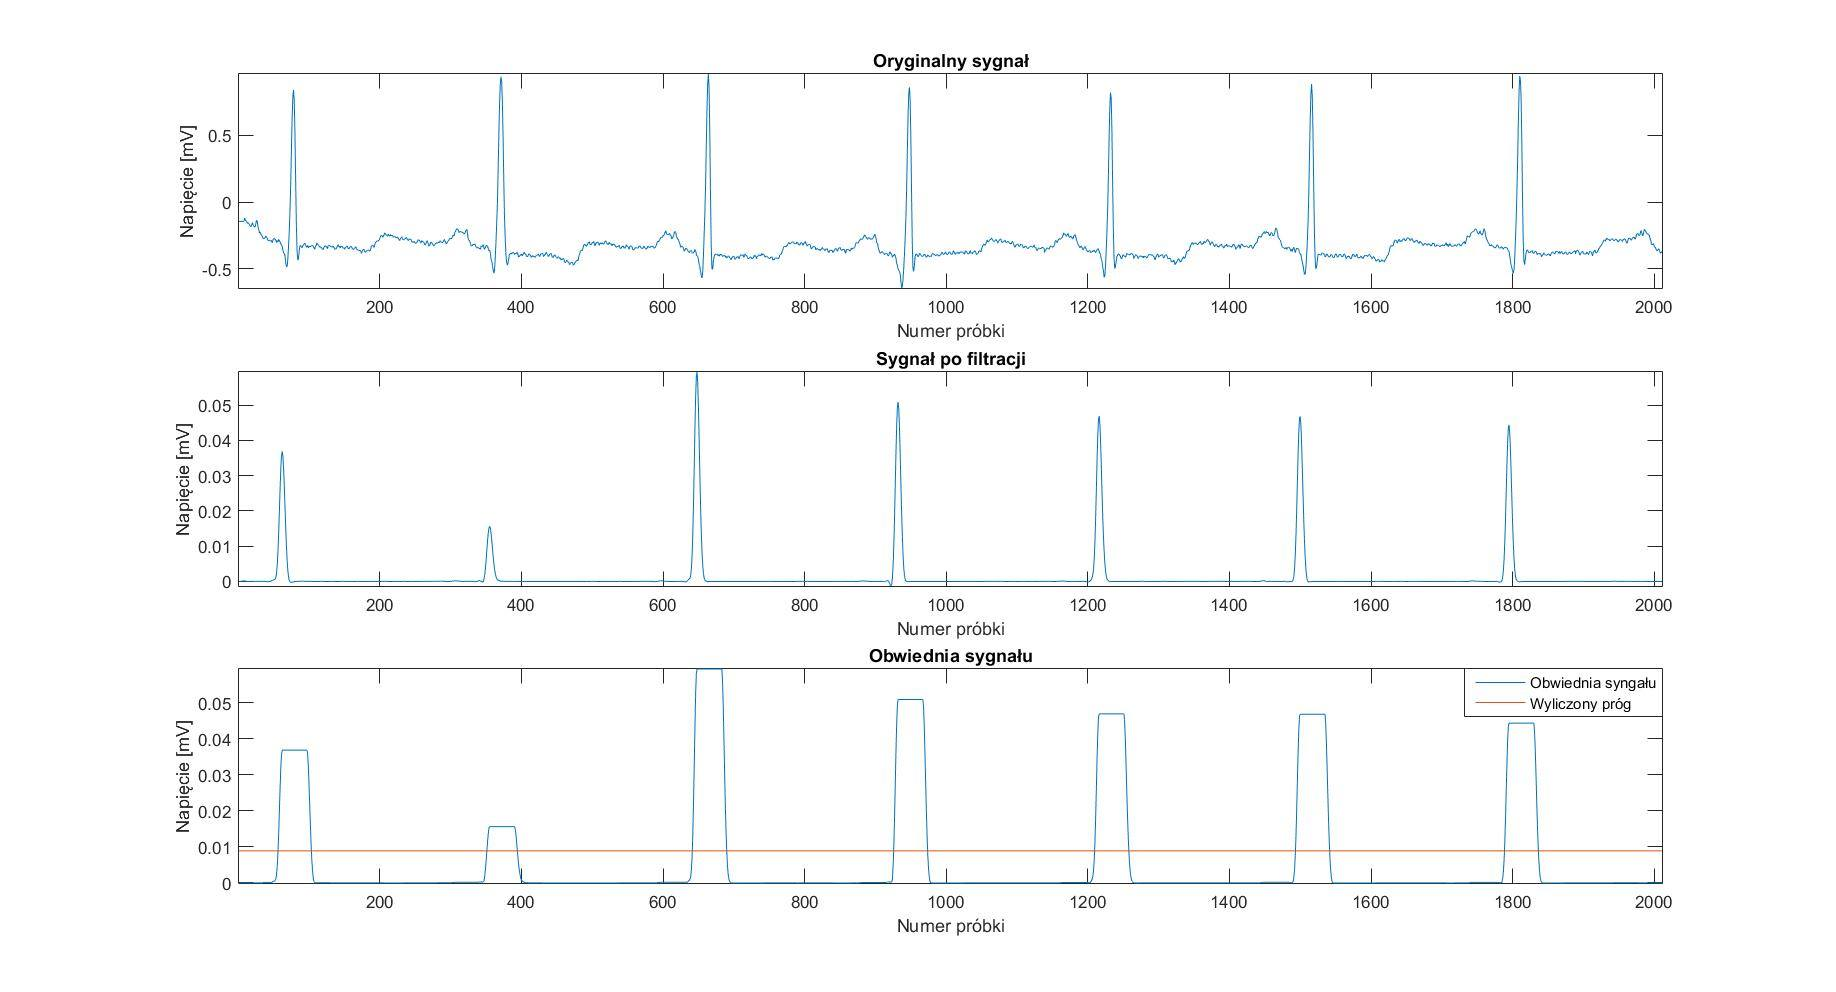
\includegraphics[width=\textwidth]{QF1}
\caption{Rezultat działania poszczególnych etapów algorytmu.}
\label{QF rys1}
\end{figure}

W rezultacie działania algorytmu generowane są numery próbek, dla których wykryto załamki R. Przykładowy wynik tego procesu, czyli oryginalny sygnał wraz z oznaczonymi załamkami przedstawiono na Rys.\ref{QF rys2}.

\medskip
\begin{figure}[h]
\centering
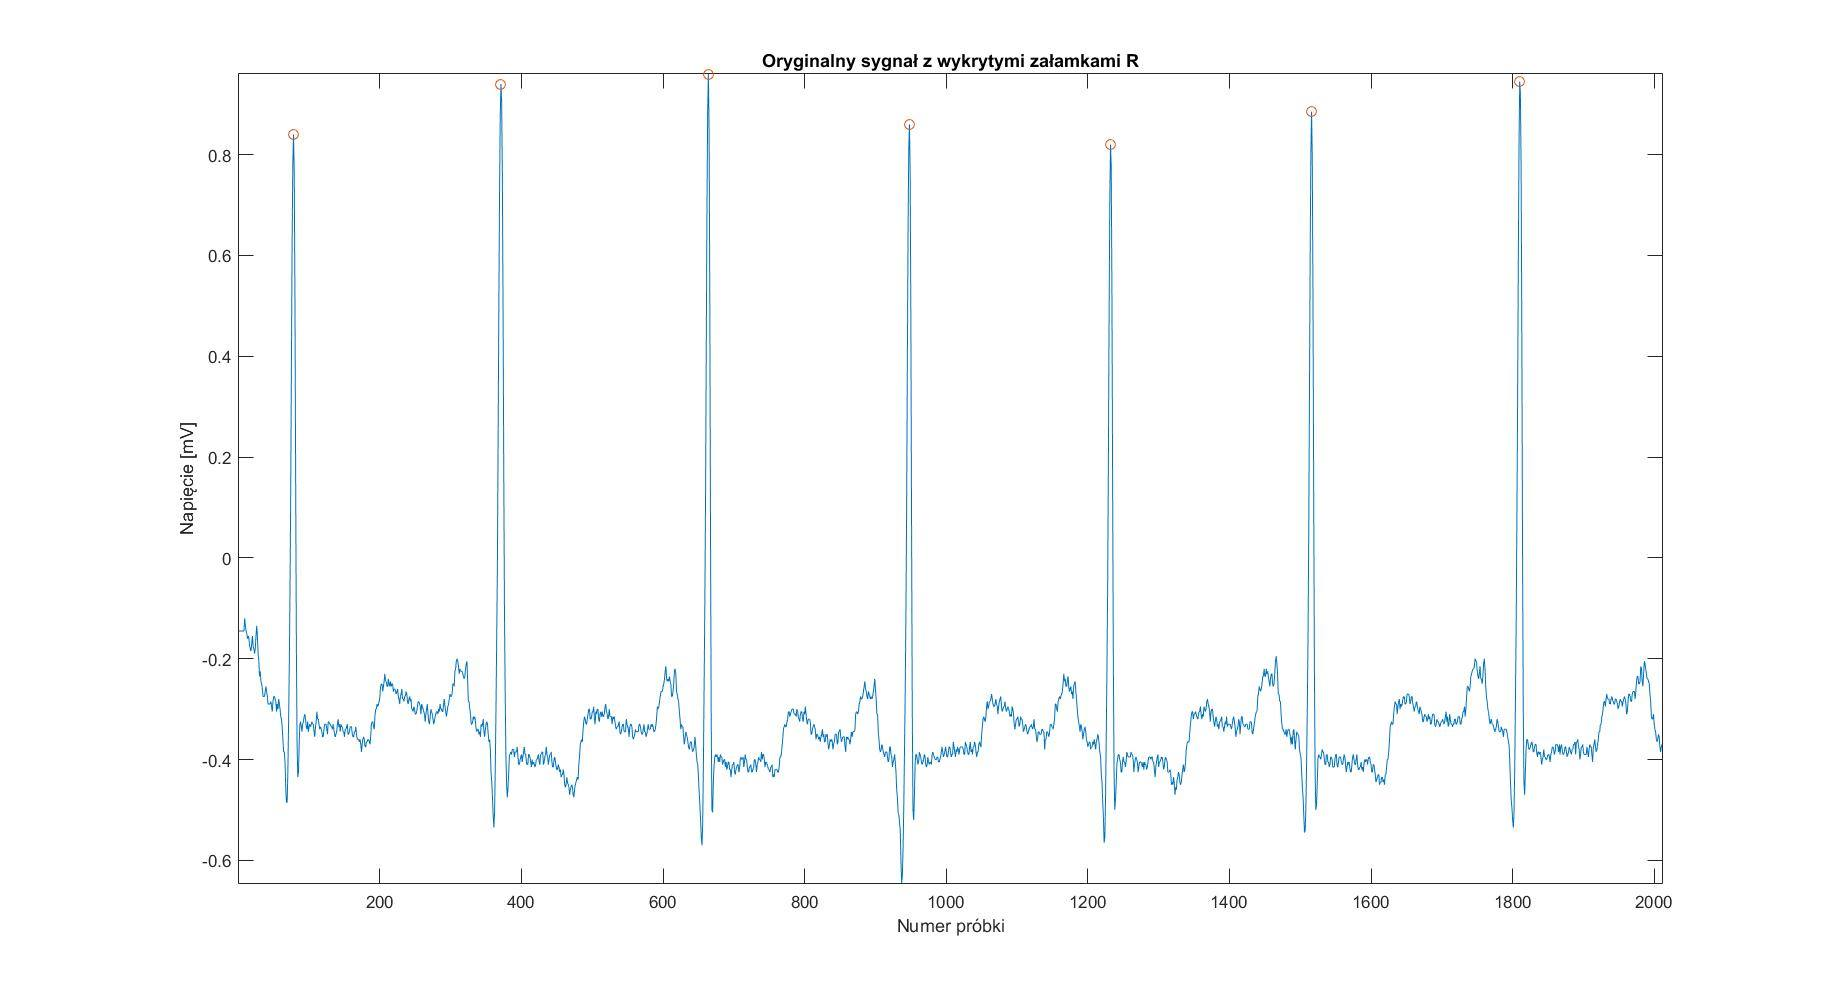
\includegraphics[width=\textwidth]{QF2}
\caption{Oryginalny sygnał wraz z oznaczonymi wykrytymi załamkami R.}
\label{QF rys2}
\end{figure}

\newpage
\subsection{Implementacja w języku C++}
\bigskip

Algorytm utworzony w języku C++ został oparty o prototyp stworzony w środowisku Matlab. Jednakże, do rozwiązania zaimplementowanego w tym języku dodano kilka części.

Pierwszą częścią programu jest wczytywanie pliku .csv. Po uruchomieniu programu użytkownik ma za zadanie wpisanie pełnej nazwy pliku, wraz z rozszerzeniem. Wybrany plik zostaje wczytany, co skutkuje pojawieniem się komunikatu "Wczytano dane z pliku". W sytuacji, gdy zostanie podana nieodpowiednia nazwa, wyświetlony zostaje odpowiedni komunikat oraz następuje zamknięcie aplikacji. Jeśli nazwa pliku została wpisana prawidłowo, program daje możliwość wyboru sygnałów, które są zapisane w tym pliku. 

Po wpisaniu oraz zatwierdzeniu wyboru sygnału, program przystępuje do obliczania macierzy współczynników filtra. Dalsze kroki algorytmu są analogiczne do opisanych w rozdziale o prototypie w środowisku Matlab.

Algorytm po kolei dokonuje filtracji sygnału z użyciem wyznaczonych współczynników, oblicza próg oraz obwiednię sygnału i ostatecznie oblicza maksima odpowiadające załamkom R. Po zakończeniu każdego z wymienionych etapów użytkownik dostaje informację w postaci komunikatu. 

Sygnał przefiltrowany, obwiednia oraz wykryte załamki są zapisywane do plików .csv. Nazwy tych plików generowane są według schematu: nazwaplikuoryginalnegoF.csv dla sygnału po filtracji, nazwaplikuoryginalnegoE.csv dla obwiedni, nazwaplikuoryginalnegoR.csv dla wykrytych załamków R.

W celu walidacji zaimplementowanego algorytmu, przetestowano go z użyciem sygnałów z bazy MIT-BIH Arrhytmia Database. Numery próbek, dla których program wykrył załamki R były konfrontowane ze wzorcami. Na tej podstawie obliczono dla każdego z sygnałów wartości parametrów: dokładności, czułości oraz precyzji. Wyniki zostały zebrane w rozdziale "Porównanie wyników".

Zaproponowany algorytm spełniał swoją funkcję i w przeważającej większości przypadków charakteryzował się skutecznością, czułością oraz precyzją na poziomie powyżej 80\%, a nawet 90\%. 

Wartość progu wyznaczana jest na podstawie parametru \begin{math}\lambda\end{math}, który powinien znajdować się w przedziale od 0.1 do 0.17, oraz maksimum sygnału. Pomimo tego, iż przyjęto najniższą możliwą wartość parametru \begin{math}\lambda\end{math}, czyli 0.1, w niektórych sygnałach detekcja nie przebiegła w sposób prawidłowy. Wiąże się to z faktem, iż w takich sygnałach występowały większe piki, przez co próg był zbyt duży.

W związku z tym, zasadna byłaby zmiana metody obliczania progu. Przykładowo, sygnał mógłby zostać podzielony na części, w których byłyby obliczane maksima. W ten sposób pojedynczy większy pik odstający od pozostałych nie wpływałby w tak istotny sposób na jakość detekcji.   

\newpage
\begin{thebibliography}{9}
\bibitem{QF article} Pornchai Phukpattaranont: \emph{QRS detection algorith based on quadratic filter}, Expert Systems with Applications, 2015, Vol. 42, Issue 11, pp. 4867-4877. 
\end{thebibliography}

\newpage
\section{Dynamic Plosion Index}

\subsection{Wprowadzenie}

Detektor zespołów QRS w sygnale elektrokardiograficznym ma za zadanie znaleźć charakterystyczne ewolucje związane z faktem depolaryzacji komór serca. Najczęściej detektory zwracają indeksy próbek sygnału, które wyznaczają wystąpienie danego zjawiska. Depolaryzacja komór jest zjawiskiem elektrofizjologicznym powodującym skurcz mięśnia sercowego oraz pompowanie krwi do aorty oraz do pnia płucnego. Algorytmom do detekcji QRS stawia się szereg założeń. Przede wszystkim powinien on oznaczać jedynie zespoły QRS. Co więcej każdy z zespołów QRS powinien być oznaczony dokładnie jeden raz. Dodatkowo wyznaczony przez detektor punkt powinien leżeć w obrębie zespołu QRS oraz dla identycznych dwóch zespołów odległość punktu od początku zespołu QRS powinna być taka sama. Analiza sygnału EKG w kontekście wyznaczania zespołów QRS jest utrudniona ze względu na możliwość wystąpienia zespołów o różnej morfologii. Częstym problemem w analizie sygnału jest również zjawisko pływania izolinii oraz przydźwięki pochodzące od sieci elektrycznej.  


Pierwotnym zastosowaniem metody Dynamic Plosion Index (DPI) była detekcja epok w sygnale mowy, która została opisana w \cite{dpi}. Metoda pozwala na wyznaczenie lokalnej cechy czasowej sygnału w oparciu o sąsiadujące próbki. Ze względu na podobieństwa dynamiki sygnału mowy oraz elektrokardiograficznego zastosowano  modyfikację DPI do wykrywania zespołów QRS. Proponowane rozwiązanie jest metodą detekcji bezprogowej. Jest to szczególnie ważne, gdy algorytm ma działać poprawnie dla różnych urządzeń i w różnych środowiskach akwizycji sygnału EKG. 

\subsection{Opis algorytmu}
Zaproponowana metoda \cite{dpi_qrs} składa się z dwóch głównych etapów. Pierwszym z nich jest wstępne przetwarzanie polegające na przefiltrowaniu EKG filtrem górnoprzepustowym oraz na jednopołówkowym wyprostowaniu sygnału (ang. \textit{half-wave}). Głównym krokiem algorytmu jest sekwencyjna lokalizacja kolejnych zespołów QRS na podstawie Dynamic Plosion Index wyliczanego od punktu należącego do poprzedniego zespołu. Schemat algorytmu przedstawiono na diagramie (Rys.\ref{schema}).
\begin{figure}[h]
    \centering
    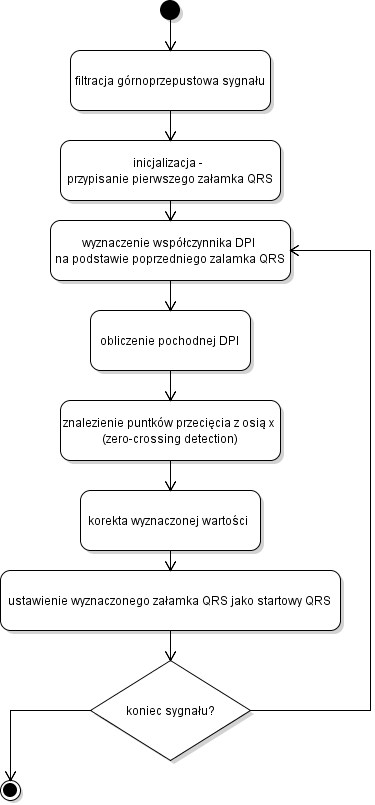
\includegraphics[width=0.4\textwidth]{img/DPI_schema.png}
    \caption{Schemat działania bezprogowego algorytmu detekcji zespołów QRS opartego o Dynamic Plosion Index}
    \label{schema}
\end{figure}

\subsubsection{Przetwarzanie wstępne sygnału}
Przed operacją właściwej detekcji zespołów QRS zazwyczaj dokonuje się filtracji pasmowo przepustowej z częstotliwościami odcięcia 8 do 20 Hz (30 Hz). Autorzy metody proponują wykorzystanie jedynie filtracji górnoprzepustowej z częstotliwością odcięcia równą 8 Hz. Zaproponowano filtrację w dziedzinie częstotliwości z wykorzystaniem narastającej funkcji cosinus w przedziale $0$ do $f_c$. Filtr w dziedzinie częstotliwości można przedstawić jako:
\begin{align}
 H(f) =
 \begin{cases}
 [0.5-0.5\cdot\cos(\pi f/f_c)]  &0\leq f \leq f_c    \\
 1 &  f_c < f \leq f_s/2
\end{cases}\
\end{align}
Filtrację górnoprzepustową zaimplementowano zarówno w środowisku MATLAB jak i w C++. Metoda filtracji w dziedzienie częstotliwości wymaga przeprowadzenia szybkiej transformaty Fouriera oraz transformacji odwrotnej. W środowisku MATLAB wykorzystano wbudowane funkcjie \textit{fft} oraz \textit{ifft}. W przypadku implemetnacji w C++ wykorzystano funkcje szybkiej transformaty Fouriera oraz transformacji odwrotnej dostępne w bibliotece Eigen. Drugim etapem wstępnego przetwarzania jest usunięcie składowych o wartościach ujemnych i pozostawienie tylko dodatnich wartości przefiltrowanego sygnału EKG. Prostowanie jednopołówkowe może wprowadzać komplikacje w przypadku ujemnego zespołu QRS, który występuje na przykład dla odprowadzenia aVR. Autorzy zakładają, że amplituda załamka S jest wówczas wystarczająca aby wyznaczyć pozycję zespołu QRS. 

\subsubsection{Plosion Index}
Plosion Index (PI) jest parametrem, który leży u podstawy opisywanej metody. Jego działanie polega na obliczeniu stosunku wartości bezwzględnej aktualnej próbki $s(n_0$) do wartości średniej próbek z zadanego przedziału ($m_1 - m_2$) \cite{dpi}. W przypadku sygnały EKG wysoka wartość współczynnika PI będzie wyznaczać miejsce poszukiwanego zespołu. Wówczas uśredniany przedział ($m_1 - m_2$) będzie zawierał próbki izolinii lub część załamka T. Formalną definicję Plosion Index można przedstawić jako:
\begin{align}
	PI(n_0,m_1,m_2) &= \frac{|s(n_0)|}{s_{avg}(n_0,m_1,m_2)} \\
	gdzie \quad s_{avg}(n_0,m_1,m_2) &= \frac{\Sigma_{i=n_0+m_1+1}^{i=n_0+m1+m_2}|s(i)|}{m_2}
\end{align}
Wartości $m_1$ oraz $m_2$ są dobierane zależnie od jakości sygnału oraz charakteru analizowanych zjawisk.
Plosion Index nie jest używany w tej postaci w przedstawianym algorytmie.
\subsubsection{Dynamic Plosion Index}
Rozwinięciem wcześniej omówionego parametru jest Dynamic Plosion Index (DPI). Można stwierdzić, że algorytm ten to sekwencje wyznaczonych współczynników PI dla następujących po sobie wartości $m_2$, przy stałej wartości $m_1$. Dodatkowo wprowadzono niewielką modyfikację równania (3). Wyliczane wartości sumy są dzielone przez $m_2^{1/p}$, co wprowadza nieliniowe skalowanie współczynników PI w funkcji odległości od punktu startowego $n_0$. Modyfikacja wprowadza wzmocnienie pików znajdujących się bliżej punktu $n_0$.
\begin{align}
 s_{avg}'(n_0,m_1,m_2) &= \frac{\Sigma_{i=n_0+m_1+1}^{i=n_0+m1+m_2}|s(i)|}{m_2^{1/p}}, p>1
\end{align}

\subsubsection{Wyznaczanie pozycji załamków QRS}
\paragraph{Inicjalizacja}
Prezentowany detektor QRS działa sekwencyjnie w oparciu o bieżącą pozycję ostatniego zespołu. W pierwszym obrocie pętli zakłada się pozycję QRS w 5 próbce sygnału. Arbitralne przypisanie pozycji pierwszego zespołu QRS jest pod koniec analizy usuwane. 
\paragraph{Wyznaczenie współczynnika DPI}
Dla zadanego okna wyliczana jest wartość współczynnika DPI. Wartość $m_1$ ustawiono na wartość -4, przy czym autorzy artykułu \cite{dpi_qrs} zaproponowali wartość -2. Oznacza to, że współczynniki DPI będą wyznaczane począwszy od zespołu QRS zawierając sam załamek R (przesunięcie o 4 próbki w lewo). Parametr $m_2$ jest wprowadzany przez użytkownika jako okno obliczeń. W przypadku analizy QRS dobrano wartość 1800ms, co odpowiada w przybliżeniu maksymalnej wartości odstępu R-R (rytm 35 uderzeń na minutę). Współczynniki DPI są wyznaczane zatem dla przedziału 0 do 1800ms na podstawie przefiltrowanego i wyprostowanego jednopołówkowo sygnału EKG. Wynikiem obliczeń jest charakterystyczny przebieg DPI w postaci kaskadowych dolin, co zostało przedstawione na Rys. \ref{dpi_plot}. 
\begin{figure}[h]
    \centering
    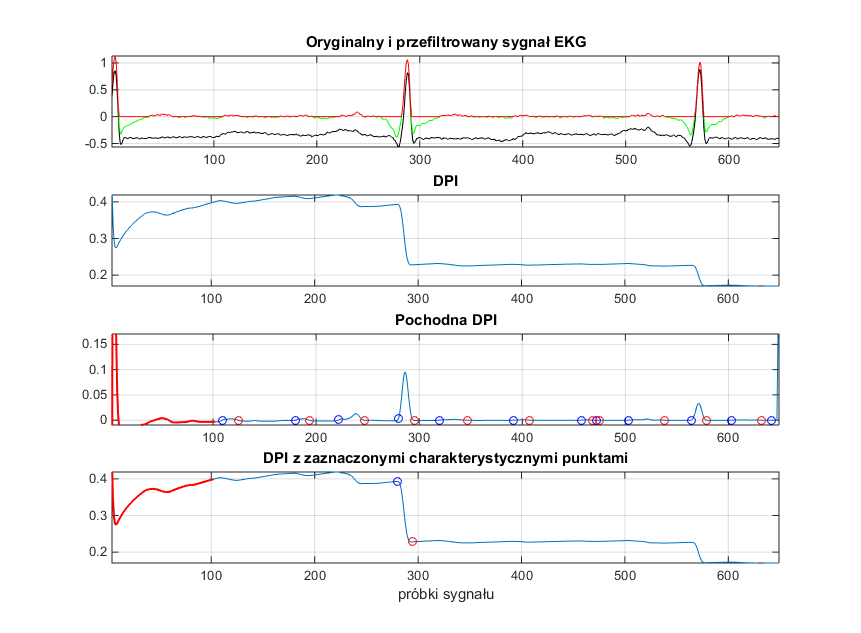
\includegraphics[width=1\textwidth]{img/DPI_single.png}
    \caption{Przebieg sygnału, parametru DPI oraz pochodnej DPI dla analizowanego okna}
    \label{dpi_plot}
\end{figure}
\newline
\textbf{Analiza pochodnej DPI}
\newline
Najważniejszy w kontekście znalezienia zespołu QRS jest wyraźny przeskok góra-dolina w DPI (ang. \textit{peak-valley}). W celu wyznaczenia lokalizacji tego obszaru wylicza się prostą pochodną DPI. Następnie wyznacza się punkty przecięcia pochodnej z zero oraz grupuje się te punkty ze względu na polaryzację zbocza (ang. \textit{positive and negative zero-crossing}). 
\paragraph{Parametr swing}
Wyznaczone ekstrema przebiegu DPI są w dalszej części analizowane w celu znalezienia maksymalnego zbocza. Wylicza się dla każdej pary punktów o dodatnim i ujemny zboczu pochodnej prosty parametr - swing. Jest on wartością bezwzględną różnicy odpowiednich wartości DPI. W ten sposób wyznacza się parę góra-dolina, która reprezentuje region występowania zespołu QRS.
\paragraph{Korekta lokalizacji QRS}
Ostatnim etapem analizy jest poprawa wyznaczonego położenia zespołu QRS na podstawie wartości bezwzględnej oryginalnego sygnału EKG przefiltrowanego górnoprzepustowo z granicą odcięcia 2 Hz. Zastosowanie wartości bezwględnej pozwala wyznaczyć położenie załamka R również w przypadku jego odwrócenia. Często w algorytmie wykorzystuje się okno o długości $\pm 285ms$, co odpowiada minimalnemu interwałowi R-R (210 uderzeń na minutę) 
Lokalizacja zespołu QRS staje się punktem startowym dla kolejnej iteracji algorytmu.

\subsection{Implementacja algorytmu}
W ramach projektu zaimplementowano prototyp algorytmu detekcji zespołów QRS z wykorzystaniem Dynamic Plosion Index w środowisku MATLAB. Wykazano w raporcie cząstkowym wysoką skuteczność oraz czułość detekcji. Kolejnym etapem była implementacja w języku C++. Ze względu na potrzebę wykonania licznych operacji macierzowych zdecydowano się wykorzystać bibliotekę Eigen \cite{eigenweb}. Podczas implementacji zwracano uwagę na wektoryzację metod. Wykorzystano system kontroli wersji Git oraz platformę Github do zarządzania projektem \cite{dpi_ecg_github}. Zaimplementowany detektor wraz z prototypem jest dostępny pod adresem: https://github.com/wegrzyn/dpi-ecg.

\subsubsection{Funkcje wejścia-wyjścia}
W pierwszej fazie wykorzystano funkcje rdsamp oraz rdann z PhysioNet  w celu przepisania plików binarnych z sygnałami do plików tekstowych. Następnie zaimplementowano w C++ funkcje odczytu plików (readRecording, readAnnotation) z sygnałami. Tworzą one wektorowe struktury danych, które następnie są przetwarzane w kolejnych krokach algorytmu. Końcowym krokiem analizy jest wyznaczenie indeksów położenia zespołów QRS. Indeksy te są zapisywane do pliku tekstowego z rozszerzeniem .dpi . 
 
\subsubsection{Funkcje pomocnicze}
W ramach implementacji algorytmu w C++ przygotowano liczne funkcje pomocnicze. Opracowano funkcję splotu (convolve), wygładzenia (smooth), prostej pochodnej (derivative). Zaimplementowano również funkcjonalność  \textit{find} czyli znalezienie indeksów wszystkich 1 w wektorze logicznym (findIndices). Opracowano również metodę znajdywania punktów przecięcia sygnału z osią 0 (zeroCrossing). Przygotowano również funkcję filtracji górnoprzepustowej w dziedzinie częstotliwości (hpf)

\subsubsection{Główne funkcjonalności}
Całość metody detekcji zespołów QRS można zrealizować wywołując funkcję dpiBasedQrsDetector. Realizuje ona wszystkie kroki algorytmu, a jej wyjściem są położenia poszukiwanych zespołów. Opracowano funkcję wyliczającą parametr swing opisany w artykule \cite{dpi}. Dodano także kilka zabiegów poprawiających położenie końcowych punktów detekcji (improveComplex). 
\newpage
\subsection{Detekcja zespołów QRS w sygnałach bazy MIT-BIH} 
Zaimplementowany algorytm został przetestowany na sygnałach pochodzących z arytmicznej bazy MIT-BIH \cite{PhysioNet}. Porównano wyznaczone punkty detekcji QRS w odniesieniu do dostępnych anotacji (Rys.\ref{208img}). Podczas porównania wykorzystano parametr okna, który określał akceptowalny błąd detekcji. Parametr ustawiono na 36 próbek, co odpowiada 100ms. Zgodnie z dokumentacją funkcji walidacyjnej bxb udostępnianej przez PhysioNet wartość ta może być zwiększona nawet do 150ms. 
\begin{figure}[h]
    \centering
    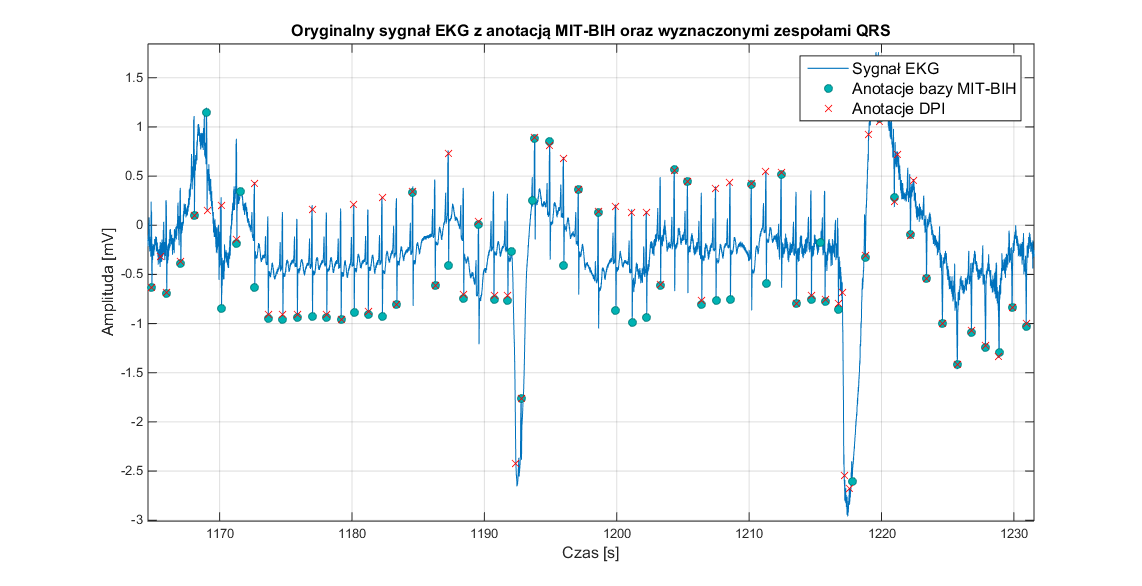
\includegraphics[width=1\textwidth]{img/208.png}
    \caption{Fragment zapisu sygnału EKG wraz z anotacją z bazy MIT-BIH oraz wyznaczonymi zespołami QRS [208.dat]}
    \label{208img}
\end{figure}
\FloatBarrier

Ze względu na specyfikę algorytmu DPI utrudnione jest znalezienie pierwszego zespołu QRS w sygnale. Dla przyjętego okna analizy warunki detekcji spełniał dopiero kolejny QRS, co można zaobserwować na Rys.\ref{beginning}. 
\begin{figure}[h]
    \centering
    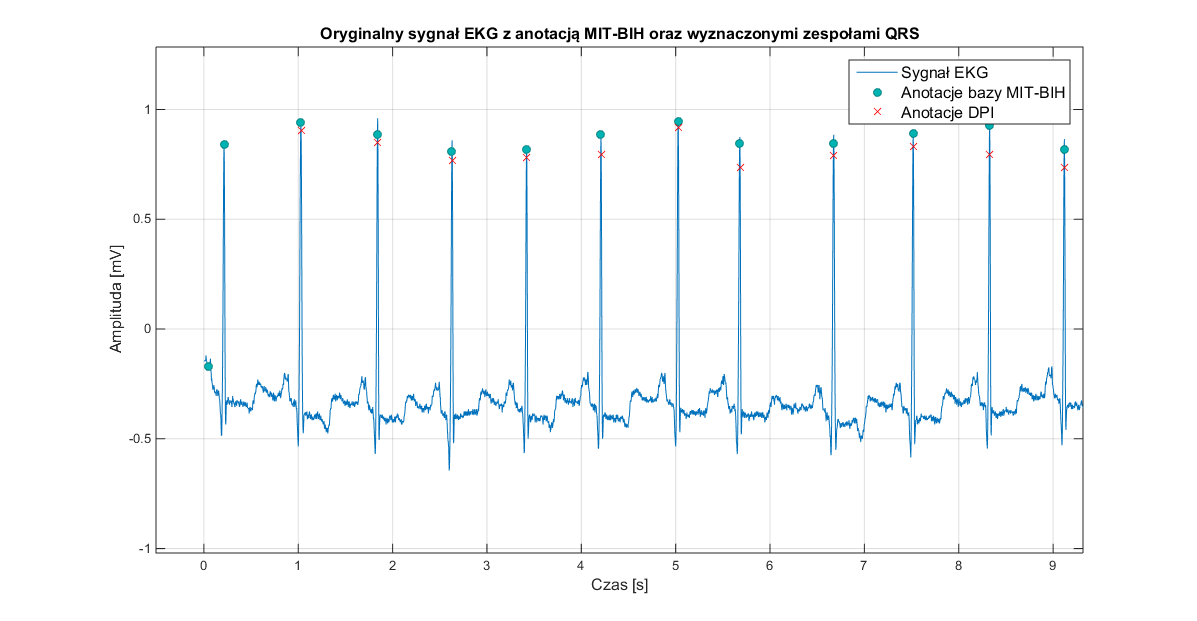
\includegraphics[width=1\textwidth]{img/100_beginning.png}
    \caption{Początkowy fragment zapisu sygnału EKG wraz z anotacją z bazy MIT-BIH oraz wyznaczonymi zespołami QRS [100.dat]}
    \label{beginning}
\end{figure}
\FloatBarrier
Można także zauważyć, że algorytm nie wykrywał dwóch ostatnich zespołów QRS sygnału elektrokardiograficznego (Rys.\ref{ending}). W założeniu metoda wymaga istnienia określonej liczby próbek w czasie sygnału ze względu na przyjęte okno analizy (1800 ms).
\begin{figure}[h]
    \centering
    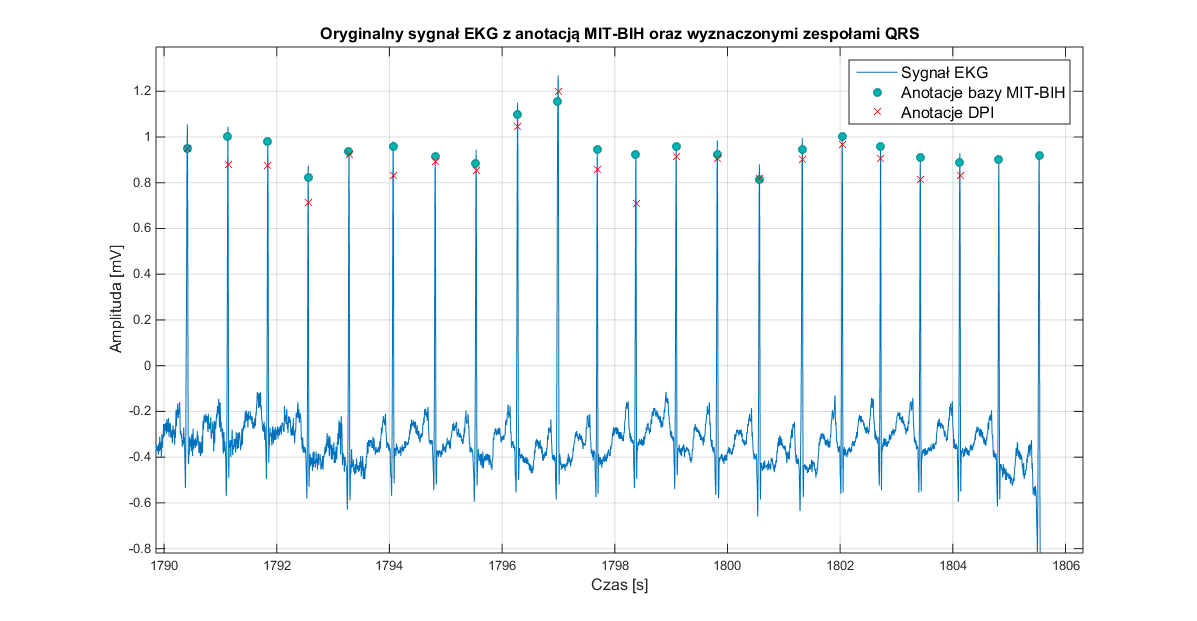
\includegraphics[width=1\textwidth]{img/100_ending.png}
    \caption{Końcowy fragment zapisu sygnału EKG wraz z anotacją z bazy MIT-BIH oraz wyznaczonymi zespołami QRS [100.dat]}
    \label{ending}
\end{figure}
\FloatBarrier

\subsection{Ocena statystyczna detektora opartego o Dynamic Plosion Index}
Dokonano również oszacowania skuteczności oraz czułości prototypu dla przykładowych sygnałów przy założeniu akceptowanego błędu równego 40 próbek. Wyniki zebrano w Tabelach 1-2.
\FloatBarrier
\begin{table}[h]
\centering
\caption{Średnia skuteczność oraz czułość detekcji dla bazy MIT-BIH}
\label{table_1}
\begin{tabular}{|c|c|c|c|}
	\hline
	Nagrania MIT-BIH & Skuteczność [\%] & Czułość[\%] & Precyzja[\%] \\
	\hline
	100 - 234 & 95,88 & 96,35 &  99,48  \\ 
	\hline
\end{tabular}
\end{table}

%\bibliographystyle{unsrt}
%\bibliography{bibliografia}
\newpage
\begin{thebibliography}{5}
\bibitem{dpi} 
A. P. Prathosh, T. V. Ananthapadmanabha, and A. G. Ramakrishnan. Epoch extraction based on
integrated linear prediction residual using plosion index. IEEE Transactions on Audio, Speech, and
Language Processing, 21(12):2471–2480, Dec 2013.

\bibitem{dpi_qrs} 
A. G. Ramakrishnan, A. P. Prathosh, and T. V. Ananthapadmanabha. Threshold-independent qrs
detection using the dynamic plosion index. IEEE Signal Processing Letters, 21(5):554–558, May 2014.
 
\bibitem{eigenweb} 
Gaël Guennebaud, Benoît Jacob, et al. Eigen v3. http://eigen.tuxfamily.org, 2010.

\bibitem{dpi_ecg_github} 
P. Wegrzynowicz and A. Zadło. dpi-ecg. https://github.com/wegrzyn/dpi-ecg, 2017.

\bibitem{PhysioNet} 
A. L. Goldberger, L. A. N. Amaral, L. Glass, J. M. Hausdorff, P. Ch. Ivanov, R. G. Mark, J. E. Mietus,
G. B. Moody, C.-K. Peng, and H. E. Stanley. Physiobank, physiotoolkit, and physionet: Components
of a new research resource for complex physiologic signals. Circulation, 101(23):e215–e220, 2000.

\end{thebibliography}


\newpage
\section{Mathematical Morphology}
\subsection{Cel projektu}

Celem projektu była implementacja algorytmu umożliwiającego wykrywanie zespołów QRS w sygnale EKG za pomocą matematycznych przekształceń morfologicznych.

\subsection{Przekształcenia morfologiczne}

Matematyczne przekształcenia morfologiczne umożliwiają analizę nieliniowego sygnału wykorzystując informacje o ich kształcie. Operacje morfologiczne wykorzystują elementy strukturalne, które najczęściej reprezentowane są przez proste kształty geometryczne, używane do detekcji sygnałów o podobnej charakterystyce. Do podstawowych przekształceń morfologicznych zalicza się operatory opisane poniżej wzorami (\ref{dylatacja}),(\ref{erozja}),(\ref{otwarcie}),(\ref{zamkniecie}) \cite{adaptiveMM}.\\

Dylatacja:
\begin{equation} 
f \oplus g(n) = max(f(n-i) + g(i))
\label{dylatacja}
\end{equation}

Erozja:
\begin{equation} 
f \ominus g(n) = min(f(n+i) - g(i))
\label{erozja}
\end{equation}

Otwarcie:
\begin{equation} 
f \circ g(n) = f \oplus g( \ominus g)(n)
\label{otwarcie}
\end{equation}

Zamknięcie:
\begin{equation} 
f \bullet g(n) = f \ominus g( \oplus g)(n)
\label{zamkniecie}
\end{equation}


\subsection{Filtracja sygnału}

W celu filtracji sygnału zastosowano filtr oparty o matematyczne przekształcenia morfologiczne. Pierwszym etapem filtracji była korekcja linii bazowej sygnału poprzez usunięcie linii dryfu z tła oryginalnego sygnału. W tym celu zastosowano przekształcenie otwarcia na sygnale wejściowym z elementem strukturalnym $B_o$ w celu usunięcia "pików" w sygnale. Kolejnym etapem było zastosowanie przekształcenia zamknięcia z elementem strukturalnym $B_c$ mające na celu usunięcie "dolin" w uzyskanym przebiegu. W wyniku opisanych przekształceń otrzymano linię dryfu $f_b$   , co opisane jest wzorem (\ref{liniadryftu}).


\begin{equation}
\ f_b = f_o \circ B_o \bullet B_c
\label{liniadryftu}
\end{equation}  

Ostatnim etapem korekcji było usunięcie linii dryfu z sygnału wejściowego, co uzyskano poprzez odjecie linii dryfu od sygnału oryginalnego, co wyraża się wzorem (\ref{korekcjald}).

\begin{equation}
\ f_{bc} = f_o - f_b
\label{korekcjald}
\end{equation}

Elementy strukturalne $B_o$,$B_c$ wykorzystane w operacji otwarcia i zamknięcia to dwie poziome linie o różnej długości, służące do detekcji linii dryfu. Długość elementów strukturalnych zależy od czasu trwania (szerokości) załamków sygnału EKG oraz częstotliwości próbkowania sygnału. Długość elementu $B_c$ musi być większa od długości elementu $B_o$. Czas trwania charakterystycznych załamków P, T, QRS jest zazwyczaj mniejszy niż 0.2s, dlatego długość elementu $B_o$ jest obliczana jako $0.2F_s$ (gdzie $F_s$ to częstotliwość próbkowania). Długość elementu $B_o$ najczęściej przyjmuje się jako $1.5L_o$ (gdzie $L_o$ to długość elementu strukturalnego $B_o$)  \cite{filtering}.\\

Kolejnym etapem filtracji było tłumienie szumu w sygnale. W tym celu zastosowano przekształcenia otwarcia i zamknięcia, a następnie uśredniono wynik. W przekształceniach wykorzystano parę elementów strukturalnych $B_{pair} = \lbrace B_1, B_2\rbrace$, gdzie $B_1 \neq B_2$. Opisane przekształcenia wyraża wzór (\ref{przeksztalceniemorf})  \cite{filtering}.

\begin{equation}
\ f = \frac{1}{2}\ (f_bc \bullet B_{pair} + f_{bc} \circ B_{pair})  = \frac{1}{2}\  (f_{bc} \oplus B_1 \ominus B_2 + f_{bc} \ominus B_1 \oplus B_2)
\label{przeksztalceniemorf}
\end{equation}

Elementy $B_1, B_2$ różnią się kształtem, ale przyjmują taką samą długość.$B_1$ ma kształt trójkąta i znajduje zastosowanie w detekcji "wzniesień" i "dolin" w sygnale takich jak np. załamki QRS. Element $B_2$ ma kształt poziomej linii i wykorzystywany jest do usuwania szumu z sygnału. W proponowanym rozwiązaniu przyjęto elementy strukturalne o długości 5 i wartościach $B_1 = (0,1,5,1,0)$ oraz $B_2 = (0,0,0,0,0)$. \\

Efekt filtracji przedstawiono na Rys. \ref{filtracja}.


\begin{figure}[h]
	\centerline{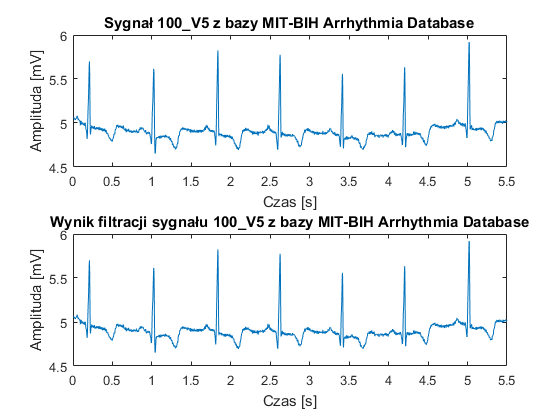
\includegraphics[scale=0.85]{filtracja}}
	\caption{ Wynik filtracji z użyciem filtru morfologicznego.}
	\label{filtracja}
\end{figure}
\FloatBarrier


\subsection{Detekcja załamków QRS}

Pierwszym etapem detekcji zespołu QRS w sygnale EKG, było wyeksponowanie "wzniesień" i "dolin" sygnału, reprezentujących załamki Q, R, S. W tym celu zastosowano kombinację transformacji Top hat i Bottom hat. Transformacja Top hat polega na odjęciu od sygnału oryginalnego wyniku operacji otwarcia tego sygnału. Pozawala to na wykrycie maksimów sygnału. Z kolei transformacja Bottom hat polega na odjęciu sygnału po jego zamknięciu. Dzięki temu wykrywa się minima \cite{MMdetection}. Połączenie tych dwóch operacji pozwala otrzymać na wyjściu wyekstrahowane cechy sygnału (maksima i minima), wskazujące miejsce występowania załamków Q, R, S \cite{adaptiveMM}. Przekształcenie wyraża się wzorem (\ref{przeksztalceniemorf2}).

\begin{equation}
\ FS = f - \frac{f \circ g + f \bullet g}{2}\ 
\label{przeksztalceniemorf2}
\end{equation}

Odpowiednio $f$ oznacza sygnał wejściowy, a $g$ element strukturalny użyty w przekształceniach morfologicznych. Kształt elementu strukturalnego $g$ dobrano tak, aby przypominał zespół QRS. W uproszczony sposób można go potraktować jako trójkąt. Szerokość elementu to czas trwania zespołu QRS mieszczący się w normie, czyli 80,6 ms. Amplituda elementu jest dobierana dla każdego sygnału indywidualnie jako różnica między maksimum i minimum znalezionym w sygnale w ciągu pierwszych 2 sekund trwania sygnału. Element strukturalny wygenerowany dla sygnału 100\_MLII z bazy MIT-BIH Database Arrythmia został pokazany na Rys. \ref{elementstrukturalny}.

\begin{figure}[h]
	\centerline{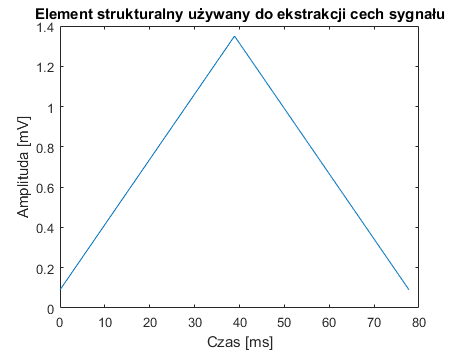
\includegraphics[scale=0.6]{element_strukturalny}}
	\caption{ Element strukturalny użyty do ekstrakcji cech.}
	\label{elementstrukturalny}
\end{figure}
\FloatBarrier

Na Rys. \ref{ekstrakcja_cech} przedstawiono schemat działania algorytmu służącego do ekstrakcji cech. Wynikiem działania przekształceń morfologicznych jest sygnał, który przedstawia jedynie wykryte "wzniesienia" i "doliny", co pokazano na Rys. \ref{e_op_morf}.

\begin{figure}[h]
	\centerline{\includegraphics[scale=0.4]{ekstrakcja_cech}}
	\caption{ Schemat działania algorytmu ekstrakcji cech.}
	\label{ekstrakcja_cech}
\end{figure}


\begin{figure}[h]
	\centerline{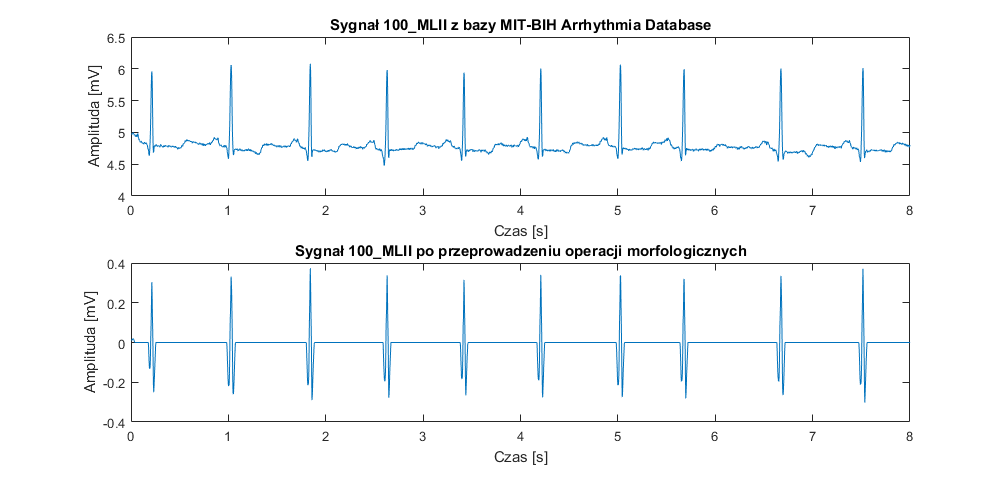
\includegraphics[scale=0.6]{efekt_operacji_morfologicznych}}
	\caption{Wynik działania przekształceń morfologicznych}
	\label{e_op_morf}
\end{figure}
\FloatBarrier

Kolejnym etapem po ekstrakcji cech sygnału była ich odpowiednia interpretacja. Wynik operacji morfologicznych nie jest całkowicie wolny od błędów. Sygnał przyjmuje wartość zero dla próbek nieleżących w obrębie zespołów QRS, a wartości dodatnie lub ujemne dla zespołów QRS. Zdarzają się jednak krótkie niezerowe sekwencje będące wynikiem zakłóceń oraz wartości równe 0 w obrębie QRS. Dlatego w pierwszym kroku wyszukiwane są sekwencje niezerowych próbek sygnału cech o długości większej niż 61 ms (zakładając czas trwania prawidłowych zespołów QRS mieści się w zakresie 60-120ms). Założono także, że w sekwencji mogą pojawić się wartości 0, ale nie więcej niż 3 pod rząd. Następnie w każdej wyznaczonej sekwencji obliczane są lokalne maksima o amplitudzie większej niż 0. Jeżeli zostanie wyznaczone pojedyncze maksimum, utożsamiane jest ono z załamkiem R, a następnie wykrywany jest załamek Q jako minimum z wartości między początkiem sekwencji a załamkiem R. W podobny sposób wykrywany jest załamek S, jako minimum z wartości między załamkiem R a końcem sekwencji. W przypadku nie wykrycia pojedynczego maksimum lokalnego, algorytm sprawdza, czy istnieją jakiekolwiek maksima w wyznaczonej sekwencji, jeżeli nie, to załamek QRS nie jest wykrywany. W przeciwnym razie jeżeli istnieją maksima lokalne to wyznaczane są załamki Q,S, a załamek R obliczany jest jako minimum z wartości pomiędzy załamkiem Q a załamkiem S. Schemat opisanej metody przedstawiony jest na Rys.\ref{schemat_decyzji}. 

\begin{figure}
	\centerline{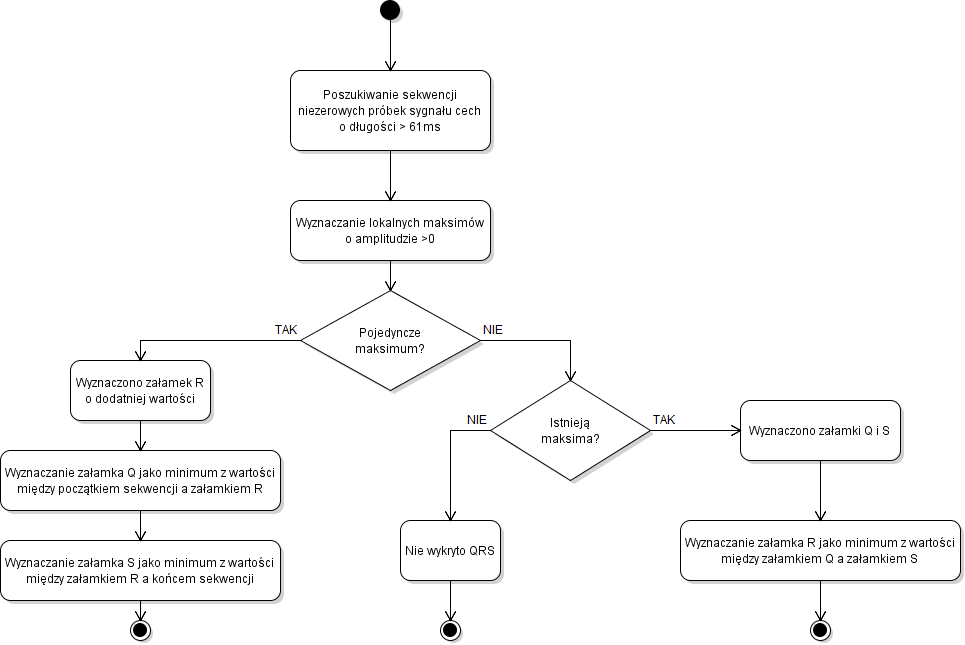
\includegraphics[scale=0.5]{pojedynczy_schemat_decyzji}}
	\caption{Schemat decyzji}
	\label{schemat_decyzji}
\end{figure}
\FloatBarrier
\newpage

\subsection{Wyniki detekcji}

W celu implementacji algorytmu do wykrywania zespołów QRS użyto środowiska MATLAB. Badane sygnały EKG pochodzą z ogólnodostępnej bazy MIT-BIH Arrhythmia Database.Poniżej na Rys.\ref{100MLII}-\ref{103V2} przedstawiono wyniki wykrywania załamków QRS metodą morfologicznych przekształceń.

\begin{figure}[h]
	\centerline{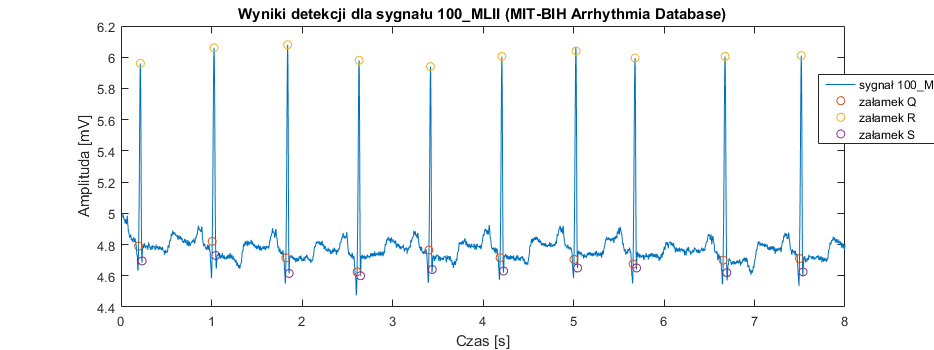
\includegraphics[scale=0.65]{100_MLII}}
	\caption{Wynik detekcji dla sygnału 100(MLII). }
	\label{100MLII}
\end{figure}

\begin{figure}[h]
	\centerline{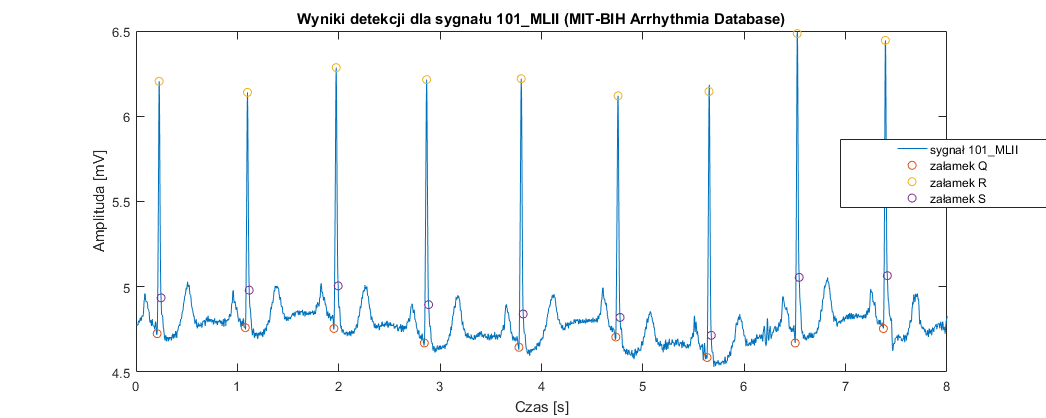
\includegraphics[scale=0.65]{101_MLII}}
	\caption{Wynik detekcji dla sygnału 101(MLII).}
	\label{101MLII}
\end{figure}

\begin{figure}[h]
	\centerline{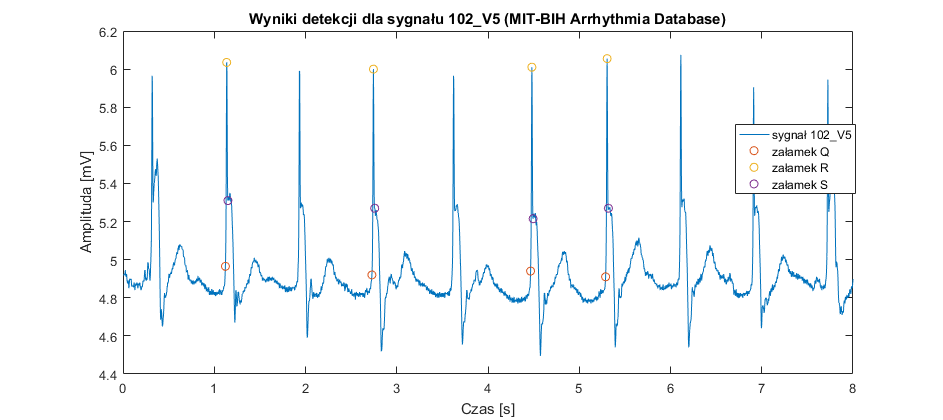
\includegraphics[scale=0.85]{102_V5}}
	\caption{Wynik detekcji dla sygnału 102(V5).}
	\label{102V5}
\end{figure}

\begin{figure}[h]
	\centerline{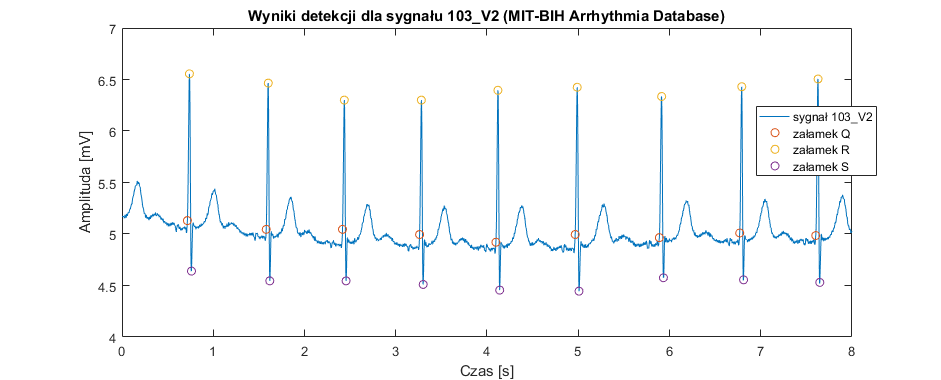
\includegraphics[scale=0.85]{103_V2}}
	\caption{Wynik detekcji dla sygnału 103(V2).}
	\label{103V2}
\end{figure}

\FloatBarrier
\newpage

\begin{thebibliography}{9}
 
\bibitem{adaptiveMM} 
S. Yazdani, J.-M. Vesin. 
\textit{Extraction of QRS fiducial points from the ECG using adaptive mathematical morphology}. 
Digital Signal Processing, 56 (2016): 100-109.

\bibitem{filtering} 
S.M. Krishnan, K.C. Keong, S. Yan, C.K. Luk.
\textit{ECG Signal Conditioning by Morphological Filters}. 
Springer 2007.
 
\bibitem{MMdetection} 
P.E. Trahanias. 
\textit{An approach to QRS complex detection using mathematical morphology}. IEEE Transactions on Biomedical Engineering 40.2 (1993): 201-205.

\end{thebibliography}

\newpage
\section{Porównanie wyników}

\bigskip
\bigskip

Dla każdego algorytmu wyznaczono wartości parametrów skuteczności, czułości oraz precyzji dla wszystkich sygnałów dostępnych w bazie MIT. Następnie wyznaczono wartości średnie oraz porównano wyżej wymienione parametry dla wszystkich algorytmów. Wyniki przedstawiono na wykresach oraz tabelach. 


Pierwszym parametrem, który porównywano była skuteczność algorytmów. Najskuteczniejszym okazał się być algorytm DynamicPlosion Index, natomiast najmniej skutecznym – Mathematical Morphology. Analogiczne wyniki skuteczności otrzymano dla sygnału 208m.mat, który ma niestandardowy przebieg. Rys.\ref{skut1} oraz \ref{skut2}.


\medskip
\begin{figure}[h!]
\centering
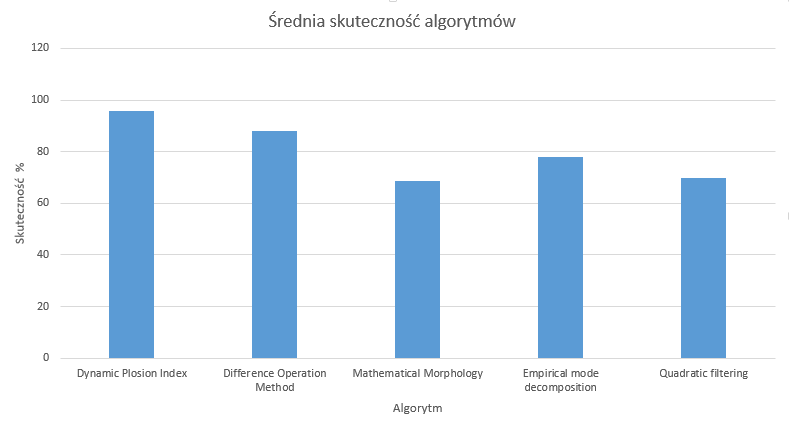
\includegraphics[width=\textwidth]{skut1}
\caption{Średnia skuteczność algorytmów [\%]. }
\label{skut1}
\end{figure} 
\FloatBarrier
\medskip

\medskip
\begin{figure}[h!]
\centering
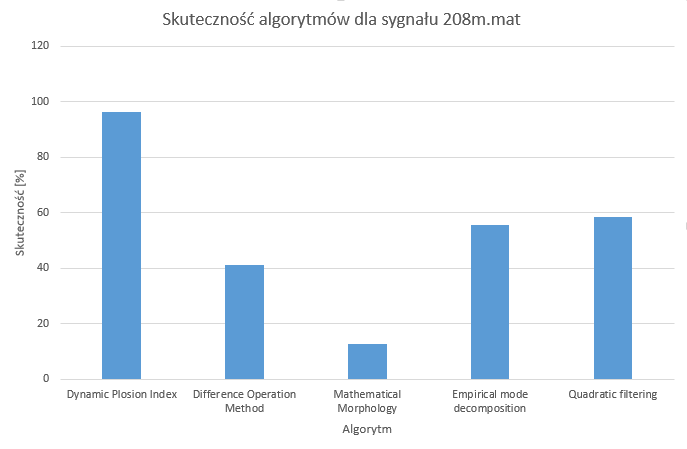
\includegraphics[width=\textwidth]{skut2}
\caption{Skuteczność algorytmów dla wybranego sygnału [\%]. }
\label{skut2}
\end{figure} 
\FloatBarrier
\medskip


Drugim parametrem, który porównywano była czułość algorytmów. Najbardziej czułym algorytmem okazał się być algorytm DynamicPlosion Index, natomiast najmniej czułym – Mathematical Morphology. Takie same wyniki czułości otrzymano dla sygnału 208m.mat. Rys.\ref{czulo1} oraz \ref{czulo2}.

\medskip
\begin{figure}[h!]
\centering
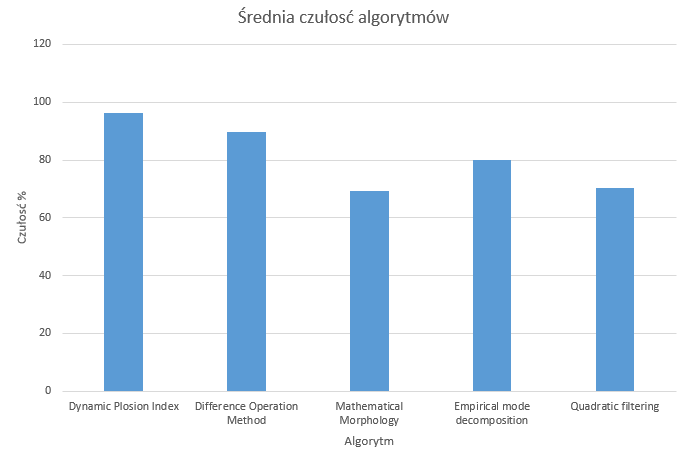
\includegraphics[width=\textwidth]{czulo1}
\caption{Średnia czułość algorytmów [\%]. }
\label{czulo1}
\end{figure} 
\FloatBarrier
\medskip

\medskip
\begin{figure}[h!]
\centering
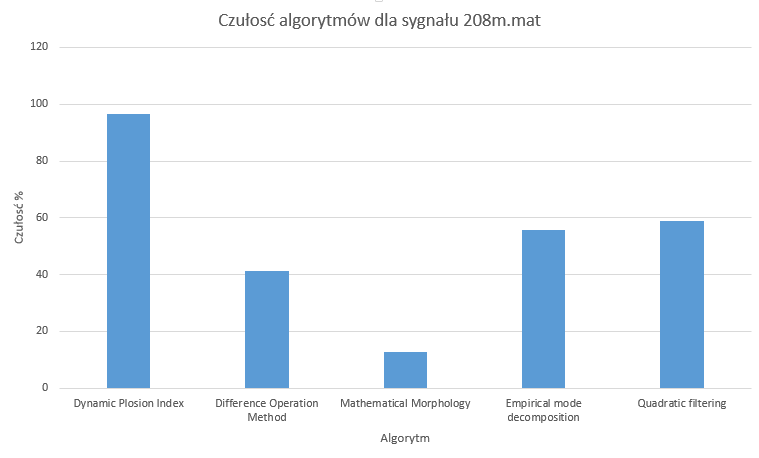
\includegraphics[width=\textwidth]{czulo2}
\caption{Czułość algorytmów dla wybranego sygnału[\%]. }
\label{czulo2}
\end{figure} 
\FloatBarrier
\medskip

Ostatnim parametrem, który porównywano była precyzja algorytmów. Najbardziej precyzyjnym algorytmem okazał się być algorytm DynamicPlosion Index, natomiast najmniej dokładnym –QuadraticFiltering. Takie same wyniki precyzji otrzymano dla sygnału 208m.mat. Rys.\ref{precis1} oraz \ref{precis2}.


\medskip
\begin{figure}[h!]
\centering
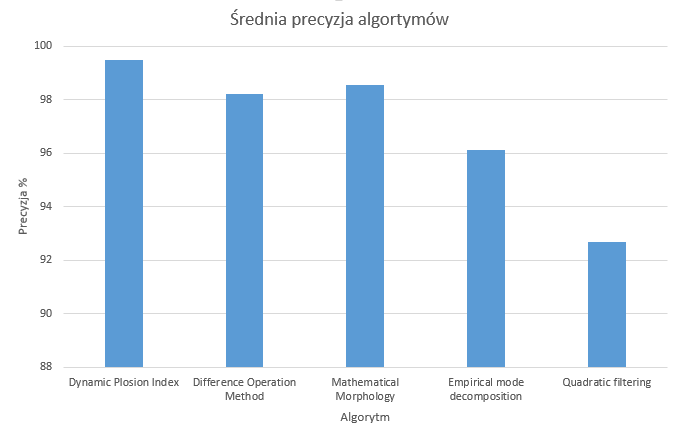
\includegraphics[width=\textwidth]{precis1}
\caption{Średnia precyzja algorytmów [\%]. }
\label{precis1}
\end{figure} 
\FloatBarrier
\medskip

\medskip
\begin{figure}[h!]
\centering
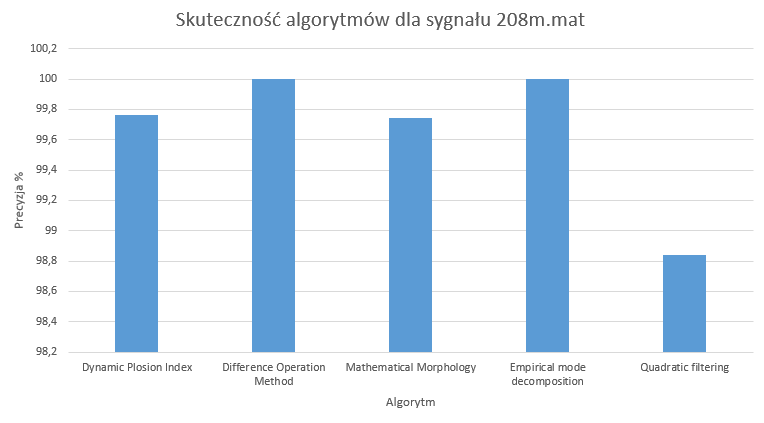
\includegraphics[width=\textwidth]{precis2}
\caption{Czułość algorytmów dla wybranego sygnału[\%]. }
\label{precis2}
\end{figure} 
\FloatBarrier
\medskip


\begin{table}
\caption{Skuteczność uzyskana dla poszczególnych sygnałów.}
\label{wynikitab1}

\centering
\resizebox{\textwidth}{!}{
\begin{tabular}{ | c | c | c | c | c | c | c |}
\hline
	MIT-BIH & Dynamic Plosion Index & Difference Operation Method & Mathematical Morphology & Empirical mode decomposition & Quadratic filtering & ŚREDNIA: \\ \hline
	100 & 99.82 & 92.86 & 99.96 & 100 & 99.47 & 98.42 \\ \hline
	101 & 99.36 & 91.67 & 99.47 & 100 & 97.31 & 97.56 \\ \hline
	102 & 99.68 & 92.31 & 18.85 & 71.43 & 94.28 & 75.31 \\ \hline
	103 & 99.62 & 91.67 & 99.43 & 100 & 99.52 & 98.05 \\ \hline
	104 & 95.69 & 92.86 & 5.68 & 16.67 & 28.57 & 47.89 \\ \hline
	105 & 94.61 & 93.33 & 93.51 & 57.14 & 0.33 & 67.78 \\ \hline
	106 & 96.38 & 83.33 & 52.12 & 100 & 68 & 79.97 \\ \hline
	107 & 97.62 & 84.62 & 70.18 & 66.67 & 95.92 & 83.00 \\ \hline
	108 & 94.39 & 61.16 & 56.74 & 66.67 & 5.9 & 56.97 \\ \hline
	109 & 99.61 & 94.44 & 94.91 & 42.86 & 10.42 & 68.45 \\ \hline
	111 & 99.44 & 92.31 & 89.73 & 100 & 65.64 & 89.42 \\ \hline
	112 & 99.45 & 93.33 & 99.29 & 100 & 33.70 & 85.15 \\ \hline
	113 & 99.34 & 90 & 99.78 & 100 & 99.94 & 97.81 \\ \hline
	114 & 97.9 & 90 & 98.52 & 100 & 98.37 & 96.96 \\ \hline
	115 & 99.54 & 90.91 & 99.44 & 100 & 99.69 & 97.92 \\ \hline
	116 & 98.72 & 86.67 & 71.42 & 100 & 98.31 & 91.02 \\ \hline
	117 & 99.68 & 90 & 26.33 & 83.33 & 96.64 & 79.20 \\ \hline
	118 & 98.91 & 92.31 & 73.13 & 14.29 & 97.41 & 75.21 \\ \hline
	119 & 94.79 & 90.91 & 0.29 & 83.33 & 94.84 & 72.83 \\ \hline
	121 & 99.09 & 90.91 & 52.48 & 83.33 & 1.74 & 65.51 \\ \hline
	122 & 99.76 & 93.75 & 99.88 & 100 & 99.92 & 98.66 \\ \hline
	123 & 99.8 & 88.89 & 99.8 & 100 & 99.8 & 97.66 \\ \hline
	124 & 98.9 & 88.89 & 93.69 & 100 & 74.56 & 91.21 \\ \hline
	200 & 93.05 & 93.75 & 40.58 & 25 & 10.02 & 52.48 \\ \hline
	201 & 94.37 & 93.33 & 92.44 & 66.67 & 92.16 & 87.79 \\ \hline
	202 & 99.11 & 90 & 98.23 & 80 & 98.47 & 93.16 \\ \hline
	203 & 86.36 & 70.37 & 24.95 & 20 & 1.5 & 40.64 \\ \hline
	205 & 98.8 & 93.75 & 98.73 & 80 & 97.49 & 93.75 \\ \hline
	207 & 84.08 & 100 & 0.59 & 50 & 0.17 & 46.97 \\ \hline
	208 & 96.42 & 41.18 & 12.63 & 55.56 & 58.37 & 52.83 \\ \hline
	209 & 95.41 & 93.75 & 96.49 & 100 & 94.28 & 95.99 \\ \hline
	210 & 94.79 & 94.12 & 55.16 & 88.89 & 0.78 & 66.75 \\ \hline
	212 & 99.38 & 93.75 & 98.84 & 62.5 & 95.7 & 90.03 \\ \hline
	213 & 98.27 & 90 & 93.65 & 90.91 & 76.05 & 89.78 \\ \hline
	214 & 97.52 & 92.31 & 35.19 & 71.43 & 43.63 & 68.02 \\ \hline
	215 & 97.79 & 90 & 97.94 & 100 & 36.56 & 84.46 \\ \hline
	217 & 96.33 & 92.31 & 0.75 & 100 & 93.61 & 76.60 \\ \hline
	219 & 92.96 & 92.86 & 88.75 & 77.78 & 92.08 & 88.89 \\ \hline
	220 & 98.74 & 100 & 51.26 & 85.71 & 99.03 & 86.95 \\ \hline
	221 & 98.34 & 78.57 & 70.05 & 71.43 & 93.42 & 82.36 \\ \hline
	222 & 91.4 & 92.86 & 62.28 & 100 & 81.94 & 85.70 \\ \hline
	223 & 98.37 & 92.86 & 56.32 & 100 & 79.15 & 85.34 \\ \hline
	228 & 88.02 & 92.31 & 90.85 & 42.86 & 1.94 & 63.20 \\ \hline
	230 & 91.36 & 87.5 & 66.86 & 88.89 & 89.05 & 84.73 \\ \hline
	231 & 77.98 & 83.33 & 77.66 & 100 & 77.81 & 83.36 \\ \hline
	232 & 83.85 & 50 & 95.87 & 80 & 95.5 & 81.04 \\ \hline
	233 & 87.79 & 78.95 & 0.38 & 22.2 & 85.55 & 54.97 \\ \hline
	234 & 99.49 & 93.75 & 99.1 & 100 & 98.7 & 98.21 \\ \hline
	ŚREDNIA: & 95.88 & 88.10 & 68.75 & 78.03 & 69.86 & 80.12 \\ \hline
\end{tabular}
}

\end{table}

\newpage

\begin{table}
\caption{Czułość uzyskana dla poszczególnych sygnałów.}
\label{wynikitab2}
\centering
\resizebox{\textwidth}{!}{\begin{tabular}{ | c | c | c | c | c | c | c |}
\hline
	MIT-BIH & Dynamic Plosion Index & Difference Operation Method & Mathematical Morphology & Empirical mode decomposition & Quadratic filtering & ŚREDNIA: \\ \hline
	100 & 99.82 & 92.86 & 99.96 & 100 & 99.52 & 98.43 \\ \hline
	101 & 99.41 & 91.67 & 99.47 & 100 & 98.61 & 97.83 \\ \hline
	102 & 99.68 & 92.31 & 18.85 & 83.33 & 94.71 & 77.78 \\ \hline
	103 & 99.62 & 91.67 & 99.43 & 100 & 99.57 & 98.06 \\ \hline
	104 & 96.15 & 92.86 & 5.71 & 16.67 & 29.39 & 48.16 \\ \hline
	105 & 95.17 & 93.33 & 94.28 & 66.67 & 0.33 & 69.96 \\ \hline
	106 & 96.38 & 83.33 & 52.12 & 100 & 68.29 & 80.02 \\ \hline
	107 & 97.62 & 84.62 & 70.3 & 100 & 96.73 & 89.85 \\ \hline
	108 & 96 & 91.67 & 56.77 & 100 & 6.09 & 70.11 \\ \hline
	109 & 99.61 & 100 & 94.91 & 42.86 & 10.46 & 69.57 \\ \hline
	111 & 99.44 & 92.31 & 89.77 & 100 & 66.14 & 89.53 \\ \hline
	112 & 99.45 & 93.33 & 99.33 & 100 & 34.09 & 85.24 \\ \hline
	113 & 99.83 & 90 & 99.78 & 100 & 99.94 & 97.91 \\ \hline
	114 & 98.52 & 90 & 98.94 & 100 & 98.73 & 97.238 \\ \hline
	115 & 99.54 & 90.91 & 99.34 & 100 & 99.64 & 97.89 \\ \hline
	116 & 99.09 & 92.86 & 71.45 & 100 & 98.64 & 92.41 \\ \hline
	117 & 99.68 & 90 & 26.33 & 100 & 97.27 & 82.66 \\ \hline
	118 & 98.91 & 92.31 & 73.13 & 14.29 & 98.09 & 75.35 \\ \hline
	119 & 94.79 & 90.91 & 0.29 & 83.33 & 94.84 & 72.83 \\ \hline
	121 & 99.15 & 90.91 & 52.48 & 83.33 & 1.76 & 65.53 \\ \hline
	122 & 99.76 & 93.75 & 99.88 & 100 & 99.92 & 98.66 \\ \hline
	123 & 99.8 & 88.89 & 99.8 & 100 & 99.8 & 97.66 \\ \hline
	124 & 98.96 & 88.89 & 93.69 & 100 & 75.38 & 91.38 \\ \hline
	200 & 93.05 & 93.75 & 46.9 & 25 & 10.21 & 53.78 \\ \hline
	201 & 95.29 & 93.33 & 92.44 & 75 & 92.25 & 89.66 \\ \hline
	202 & 99.11 & 90 & 98.23 & 80 & 98.93 & 93.25 \\ \hline
	203 & 86.36 & 86.36 & 28.81 & 20 & 1.51 & 44.61 \\ \hline
	205 & 98.8 & 93.75 & 98.61 & 100 & 97.45 & 97.72 \\ \hline
	207 & 85.91 & 100 & 0.59 & 50 & 0.17 & 47.33 \\ \hline
	208 & 96.64 & 41.18 & 12.64 & 55.56 & 58.77 & 52.96 \\ \hline
	209 & 95.41 & 93.75 & 96.49 & 100 & 95.61 & 96.25 \\ \hline
	210 & 94.79 & 94.12 & 55.18 & 88.89 & 0.78 & 66.75 \\ \hline
	212 & 99.38 & 93.75 & 98.84 & 62.5 & 97.47 & 90.39 \\ \hline
	213 & 98.27 & 94.74 & 93.65 & 100 & 78.01 & 92.93 \\ \hline
	214 & 97.56 & 92.31 & 35.19 & 7.43 & 43.73 & 55.24 \\ \hline
	215 & 97.79 & 94.74 & 97.91 & 100 & 36.57 & 85.40 \\ \hline
	217 & 96.62 & 92.31 & 0.75 & 100 & 94.43 & 76.82 \\ \hline
	219 & 93.12 & 92.86 & 88.75 & 100 & 92.12 & 93.37 \\ \hline
	220 & 98.74 & 100 & 51.26 & 85.71 & 99.03 & 86.95 \\ \hline
	221 & 98.42 & 78.57 & 70.05 & 71.43 & 93.5 & 82.39 \\ \hline
	222 & 92.03 & 92.86 & 62.21 & 100 & 82.87 & 85.994 \\ \hline
	223 & 98.37 & 92.86 & 65.32 & 100 & 79.18 & 87.15 \\ \hline
	228 & 88.23 & 92.31 & 93.27 & 42.86 & 1.96 & 63.73 \\ \hline
	230 & 91.36 & 87.5 & 66.86 & 88.89 & 89.37 & 84.80 \\ \hline
	231 & 78.17 & 83.33 & 77.66 & 100 & 77.81 & 83.39 \\ \hline
	232 & 97.8 & 50 & 95.92 & 80 & 97.14 & 84.17 \\ \hline
	233 & 87.79 & 83.33 & 0.38 & 22 & 87.15 & 56.12 \\ \hline
	234 & 99.49 & 93.75 & 99.1 & 100 & 98.95 & 98.25 \\ \hline
	ŚREDNIA: & 96.35 & 89.60 & 69.23 & 80.12 & 70.27  \\ \hline
\end{tabular}
}

\end{table}

\newpage

\begin{table}
\caption{Precyzja uzyskana dla poszczególnych sygnałów.}
\label{wynikitab3}
\centering
\resizebox{\textwidth}{!}{\begin{tabular}{ | c | c | c | c | c | c | c |}

\hline
	MIT-BIH & Dynamic Plosion Index & Difference Operation Method & Mathematical Morphology & Empirical mode decomposition & Quadratic filtering & ŚREDNIA: \\ \hline
	100 & 100 & 100 & 100 & 100 & 99.96 & 99.99 \\ \hline
	101 & 99.95 & 100 & 100 & 100 & 98.66 & 99.72 \\ \hline
	102 & 100 & 100 & 100 & 83.33 & 99.52 & 96.57 \\ \hline
	103 & 100 & 100 & 100 & 100 & 99.95 & 99.99 \\ \hline
	104 & 99.51 & 100 & 91.03 & 100 & 91.02 & 96.31 \\ \hline
	105 & 99.38 & 100 & 99.14 & 80 & 60 & 87.7 \\ \hline
	106 & 100 & 100 & 100 & 100 & 99.38 & 99.88 \\ \hline
	107 & 100 & 100 & 91.24 & 66.7 & 99.14 & 91.42 \\ \hline
	108 & 98.26 & 64.71 & 99.98 & 66.7 & 65.29 & 78.99 \\ \hline
	109 & 100 & 94.44 & 100 & 100 & 97.07 & 98.3 \\ \hline
	111 & 100 & 100 & 99.95 & 100 & 98.88 & 99.77 \\ \hline
	112 & 100 & 100 & 99.96 & 100 & 96.66 & 99.32 \\ \hline
	113 & 99.5 & 100 & 100 & 100 & 100 & 99.9 \\ \hline
	114 & 99.36 & 100 & 99.57 & 100 & 99.63 & 99.71 \\ \hline
	115 & 100 & 100 & 100 & 100 & 100 & 100 \\ \hline
	116 & 99.63 & 92.86 & 99.94 & 100 & 99.67 & 98.42 \\ \hline
	117 & 100 & 100 & 100 & 83.33 & 99.34 & 96.53 \\ \hline
	118 & 100 & 100 & 100 & 100 & 99.3 & 99.86 \\ \hline
	119 & 100 & 100 & 100 & 100 & 100 & 100 \\ \hline
	121 & 99.95 & 100 & 100 & 100 & 55.93 & 91.18 \\ \hline
	122 & 100 & 100 & 100 & 100 & 100 & 100 \\ \hline
	123 & 100 & 100 & 100 & 100 & 100 & 100 \\ \hline
	124 & 99.94 & 100 & 100 & 100 & 98.56 & 99.7 \\ \hline
	200 & 100 & 100 & 75.06 & 100 & 84.32 & 91.88 \\ \hline
	201 & 98.98 & 100 & 100 & 85.71 & 99.89 & 96.92 \\ \hline
	202 & 100 & 100 & 100 & 100 & 99.53 & 99.91 \\ \hline
	203 & 100 & 79.17 & 100 & 100 & 63.51 & 88.54 \\ \hline
	205 & 100 & 100 & 100 & 80 & 100 & 96 \\ \hline
	207 & 97.52 & 100 & 77.78 & 100 & 33.33 & 81.73 \\ \hline
	208 & 99.76 & 100 & 99.74 & 100 & 98.84 & 99.67 \\ \hline
	209 & 100 & 100 & 100 & 100 & 98.55 & 99.71 \\ \hline
	210 & 100 & 100 & 99.93 & 100 & 61.76 & 92.34 \\ \hline
	212 & 100 & 100 & 100 & 100 & 98.14 & 99.63 \\ \hline
	213 & 100 & 94.74 & 100 & 90.91 & 96.8 & 96.49 \\ \hline
	214 & 99.96 & 100 & 100 & 100 & 99.5 & 99.89 \\ \hline
	215 & 100 & 94.74 & 100 & 100 & 99.92 & 98.93 \\ \hline
	217 & 99.68 & 100 & 100 & 100 & 99.08 & 99.75 \\ \hline
	219 & 99.81 & 100 & 100 & 77.78 & 99.95 & 95.51 \\ \hline
	220 & 100 & 100 & 100 & 100 & 100 & 100 \\ \hline
	221 & 99.92 & 100 & 100 & 100 & 99.91 & 99.97 \\ \hline
	222 & 99.26 & 100 & 100 & 100 & 98.64 & 99.58 \\ \hline
	223 & 100 & 100 & 100 & 100 & 99.95 & 99.99 \\ \hline
	228 & 99.74 & 100 & 97.22 & 100 & 63.64 & 92.12 \\ \hline
	230 & 100 & 100 & 100 & 100 & 99.59 & 99.92 \\ \hline
	231 & 99.68 & 100 & 100 & 100 & 100 & 99.94 \\ \hline
	232 & 85.47 & 100 & 99.94 & 100 & 98.27 & 96.74 \\ \hline
	233 & 100 & 93.75 & 100 & 100 & 97.9 & 98.33 \\ \hline
	234 & 100 & 100 & 100 & 100 & 99.74 & 99.95 \\ \hline
	ŚREDNIA: & 99.48 & 98.22 & 98.55 & 96.13 & 92.68 &  \\ \hline

\end{tabular}
}

\end{table}





\end{document}